\documentclass[a4paper,11pt]{article}
\usepackage[table]{xcolor}



\newcommand{\defeq}{\mathrel{\doteq}}

\newcommand{\lzero}{0}

\newcommand{\kw}[1]{\mathtt{#1}}

\newcommand{\expr}{e}
\newcommand{\vall}{w}
\newcommand{\valr}{v}
\newcommand{\eif}{\kw{if}}
\newcommand{\eapp}{\;}
\newcommand{\eprojl}{\kw{fst}}
\newcommand{\eprojr}{\kw{snd}}
%\newcommand{\eprov}[1]{\eta_{#1}}
\newcommand{\etrue}{\kw{true}}
\newcommand{\efalse}{\kw{false}}
\newcommand{\econst}{c}
\newcommand{\eop}{\delta}
\newcommand{\efix}{\mathop{\kw{fix}}}
%\newcommand{\labelA}{\ell}

\newcommand{\tr}{T}
\newcommand{\trift}{\eif^{\kw{t}}}
\newcommand{\triff}{\eif^{\kw{f}}}
\newcommand{\trprojl}{\eprojl}
\newcommand{\trprojr}{\eprojr}
\newcommand{\trtrue}{\etrue}
\newcommand{\trfalse}{\efalse}
\newcommand{\trconst}{\econst}
\newcommand{\trop}{\eop}
\newcommand{\trfix}{\efix}
\newcommand{\trapp}[5]{#1 \; #2 \mathrel{\triangleright} {\efix #3(#4).#5}}

\newcommand{\adap}{\kw{adap}}
\newcommand{\ddep}[1]{\kw{depth}_{#1}}
\newcommand{\nat}{\mathbb{N}}
\newcommand{\natb}{\nat_{\bot}}
\newcommand{\natbi}{\natb^\infty}
\newcommand{\nnatA}{n}
\newcommand{\nnatB}{m}
\newcommand{\nnatbA}{s}
\newcommand{\nnatbB}{t}
\newcommand{\nnatbiA}{q}
\newcommand{\nnatbiB}{r}

\newcommand{\type}{\tau}
\newcommand{\tbase}{\kw{b}}
\newcommand{\tbool}{\kw{bool}}
\newcommand{\tarr}[5]{#1; #3 \xrightarrow{#4; \, #5} #2}
\newcommand{\env}{\theta}

\newcommand{\bigstep}{\mathrel{\Downarrow}}

\newcommand{\dmap}{\rho}
\newcommand{\dmapb}{\bot_\dmap}
\newcommand{\supp}{\kw{supp}}
\newcommand{\dom}{\kw{dom}}

\newcommand{\tvdash}[1]{\vdash_{#1}}

%Packages
\usepackage[T1]{fontenc}
\usepackage{fourier} 
\usepackage[english]{babel} 
\usepackage{amsmath,amsfonts} 
\usepackage{amsthm} 
\usepackage{color}   %May be necessary if you want to color links
\usepackage{hyperref}
\usepackage{lscape}
\usepackage{geometry}
\usepackage{amsmath}
\usepackage{algorithm}
\usepackage{algorithmic}
\usepackage{amssymb}
\usepackage{amsfonts}
\usepackage{times}
\usepackage{bm}
\usepackage{ stmaryrd }
\SetSymbolFont{stmry}{bold}{U}{stmry}{m}{n}

\usepackage{ amssymb }
\usepackage{ textcomp }
\usepackage[normalem]{ulem}
% For derivation rules
\usepackage{mathpartir}
\usepackage{color}
\usepackage{a4wide}
\usepackage{caption}
\usepackage{subcaption}
\usepackage{mathpartir}
\usepackage{amsmath,amsfonts}
\usepackage{ amssymb }
\usepackage{color}
\usepackage{algorithm}
\usepackage{algorithmic}
\usepackage{microtype}
\usepackage{eucal}
\usepackage{url}
\usepackage{xspace}
\usepackage{array}
\usepackage{listings}

\usepackage{tikz}
\usetikzlibrary{shapes.geometric}
\usetikzlibrary{arrows.meta,arrows}
\usetikzlibrary{decorations.text}
% % % % 


\usepackage{multirow}


%%%%%%%%%%%%%%%%%%%%%%%%%%%%%%%%%%%%%%%%%%%%%%%%%%%%%Packages And Definitions For Listing the Code%%%%%%%%%%%%%%%%%%%%%%%%%%%%%%%%%%%%%%%%%%%%%%%%%%%%%%%%%%%%%%%%%%%%%%%%
\usepackage{listings}
\usepackage{xcolor}

\definecolor{codegreen}{rgb}{0,0.6,0}
\definecolor{codegray}{rgb}{0.5,0.5,0.5}
\definecolor{codepurple}{rgb}{0.58,0,0.82}
\definecolor{backcolour}{rgb}{0.95,0.95,0.92}

\lstdefinestyle{mystyle}{
    backgroundcolor=\color{backcolour},   
    commentstyle=\color{codegreen},
    keywordstyle=\color{magenta},
    numberstyle=\tiny\color{codegray},
    stringstyle=\color{codepurple},
    basicstyle=\ttfamily\footnotesize,
    breakatwhitespace=false,         
    breaklines=true,                 
    captionpos=b,                    
    keepspaces=true,                 
    numbers=left,                    
    numbersep=5pt,                  
    showspaces=false,                
    showstringspaces=false,
    showtabs=false,                  
    tabsize=2
}

\lstset{style=mystyle}

\usepackage{tikz}
\usetikzlibrary{shapes,arrows}
\newcommand{\THESYSTEM}{\textsf{AdaptFun}}

% Define block styles
\tikzstyle{decision} = [diamond, draw, fill=blue!20, 
    text width=4.5em, text badly centered, node distance=3cm, inner sep=0pt]
\tikzstyle{block} = [rectangle, draw, fill=blue!20, 
    text width=5em, text centered, rounded corners, minimum height=4em]
\tikzstyle{line} = [draw, -latex']
\tikzstyle{cloud} = [draw, ellipse,fill=red!20, node distance=3cm,
    minimum height=2em]

\begin{document}
\title{Adaptivity Analysis}

\author{}

\date{}

\maketitle

\begin{abstract}
  A data analysis is said to \emph{generalize} when it allows one to draw
  conclusions from the data that are true of the population from which
  the data are sampled. Statistician and data scientist have devised
  several methods aimed to guarantee generalization in  data
  analyses, and avoid in this way overfitting to the
  data. Guaranteeing generalization is more difficult when data
  analyses are \emph{adaptive}: when the result of an analysis depends
  on the result of previous analyses. 

  A recent line of work focuses on methods aimed at guaranteeing
  generalization in adaptive data analysis through the addition of
  carefully calibrated statistical noise to the empirical results of
  the analysis on the sampled data. In these works, the confidence
  intervals on the generalization error that one can achieve for a
  given analysis usually depend on the \emph{level of adaptivity} of
  the analysis: the number of adaptive steps that depend on
  each other. 

  In this work we introduce a programming framework, named \THESYSTEM,  aimed at
  supporting the study of the generalization error for adaptive data
  analysis. Through its analysis system, an upper bound on the
  adaptivity -- depth (the length of the longest chain of queries) of
  a program implementing an adaptive data analysis can be overestimated. We show how this language can help to analyze the generalization error between two data analyses with different adaptivity structures.
\end{abstract}

\tableofcontents


% \section{Introduction}
\section{System Overview}
In adaptive data analysis, a data analysis can depend on the results of
previous analysis over the same data. This dependency may affect the
\emph{generalization properties of the data analysis}. To study this phenomenon
in a formal way, we consider the \emph{statistical query
  model}. In this model, a dataset $X$ consisting of $d$ attributes (columns) and $n$
individuals' data (rows) can be accessed only through an interface to
which one can submit statistical queries. More precisely, suppose that
the type of a row is $R$ (as an example, a row with $d$ binary
attributes would have type $R=\{0,1\}^d$. Then, in the statistical
query model one can access the dataset only by submitting a query to
the interface, in
the form of a function
$p:D\to [0,1] $ where $D$ represents dataset. The collected answer of
the asked query is the average result of $p$ on each row in the
dataset $D$. For example, the result is the
value $\frac{1}{n}\sum_{i=1}^n p(X_i)$ where
$X_i$ is the row of index $i$ in $X$. While this model is rather
simple, in fact it supports sufficient statistics one may be
interested.
\begin{figure}
    \centering    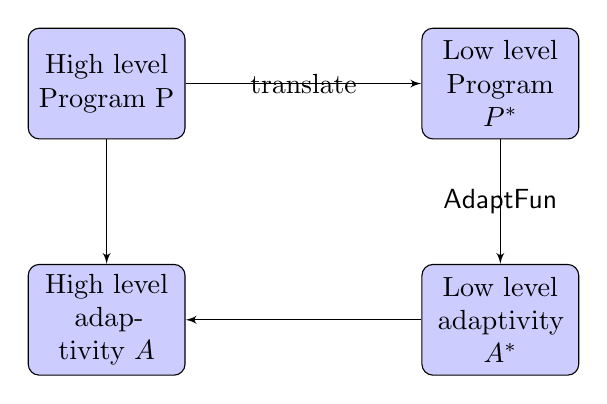
\begin{tikzpicture}{node distance = 2cm, auto}
  % nodes
  \node [block](high){High level Program P } ;
  \node [block, right of = high, node distance = 5cm](low){Low level Program $P^*$  } ;
  \node [block, below of = low, node distance = 3cm](adaptlow){Low level adaptivity $A^*$};
   \node [block, below of = high, node distance = 3cm](adapthigh){High level adaptivity $A$};
  % edges
  \path [line] (high) -- node {translate} (low) ;
  \path [line] (low) -- node {\THESYSTEM}(adaptlow);
  \path [line] (adaptlow) -- (adapthigh) ;
  \path [line]  (high) -- (adapthigh);   
 \end{tikzpicture} 
    \caption{High level architecture}
    \label{fig:structure}
\end{figure}

% \begin{tikzpicture}[node distance = 2cm, auto]
%     % Place nodes
%     \node [block] (init) {initialize model};
%     \node [cloud, left of=init] (expert) {expert};
%     \node [cloud, right of=init] (system) {system};
%     \node [block, below of=init] (identify) {identify candidate models};
%     \node [block, below of=identify] (evaluate) {evaluate candidate models};
%     \node [block, left of=evaluate, node distance=3cm] (update) {update model};
%     \node [decision, below of=evaluate] (decide) {is best candidate better?};
%     \node [block, below =decide, node distance=3cm] (stop) {stop};
%     % Draw edges
%     \path [line] (init) -- (identify);
%     \path [line] (identify) -- (evaluate);
%     \path [line] (evaluate) -- (decide);
%     \path [line] (decide) -| node [near start] {yes} (update);
%     \path [line] (update) |- (identify);
%     \path [line] (decide) -- node {no}(stop);
%     \path [line,dashed] (expert) -- (init);
%     \path [line,dashed] (system) -- (init);
%     \path [line,dashed] (system) |- (evaluate);
%   \end{tikzpicture}
 

We are interested in the adaptivity of mechanisms in the model, which is straightforward supported by a high level language. In this language, queries are allowed to carry arguments to simulate the process of submitting a query to the interface in
the model, for example, the expression $q(e)$ tells us the argument $e$ is consumed to construct the
query. To be precise, one submitted query who needs the average of
answers of previous queries is expressed as $q(x)$, where the variable $x$ stores
the expected average results.This makes these mechanisms quite straightforward to express in the high level language. However, this convenience pays at the price that the adaptivity $A$ of a mechanism $P$ becomes quite tricky to estimate because the definition of dependency between two queries becomes vague in the high level language. 

\[
\begin{array}{l}
     x \leftarrow q_1() ; \\
    \eif \; (x_1 > 0 )\; \\
     y \leftarrow q_2(x) \; \\
    % \mathsf{else} \; \left[y_2 \leftarrow 0 \right]^4; \\
    % \eif \; \left[x_1 \right]^5\; \\
    % \mathsf{then} \; \left[ y_3 \leftarrow 0 \right]^6\; \\
    % \mathsf{else} \; \left[y_4 \leftarrow q_2 \right]^7; \\
\end{array}
\]

The dependency between two query submissions is the essential of the adaptivity of a mechanism. To study the dependency, we first study its dual, independence between two queries, which is defined to be: one query
$q_1$ does not
depend on another query $q_2$ when the result of $q_1$ remains the
same regardless of the modification of the result of $q_2$. Hence, it becomes hard to distinguish whether the variance of result of $q_1$ comes from the control flow or the argument of queries. Since we know that the result of one query from a specific $D$ may vary under different contexts in the high level language.  




% Nevertheless, in \emph{statistical query
%   model},  Our definition of the dependency lies
% in the independence between two queries: one query
% $q_1$ does not
% depend on another query $q_2$ when the result of $q_1$ remains the
% same regardless of the modification of the result of $q_2$. Following such
% definition, the dependency between two queries comes from either the
% control flow or the argument of the function $q_2$, which brings us
% difficulty to distinguish them at the semantic level. \\
% {An example to show how do control flow and query argument may bring challenges}.

To resolve the dilemma, shown in Fig~\ref{fig:structure}, we translate any program(mechanism) into its counterpart in a low level language, which mimics the high level one except its only allowing atomic queries, -- $q$ --. That is to say, given a data base $D$, the result of the
query from $D$ becomes deterministic. We need to show the two programs $P$ and $P^*$ are observably equivalent over the translation. In this way, we can define the adaptivity of
a program under this model only based on the control flow.
To be specific, the adaptivity $A^*$ of a low level program $P^*$ is defined by
graphs, called dependency graph, which comes from the semantics of the low level program. The dependency graph is constructed using a
trace of queries generated along with the semantics: The queries in the trace consists of the nodes in the graph
while the edge represents dependency. If there is no dependency between
two node(queries), there will be no edge. Intuitively, we want to give an over-approximate of $A^*$ by static analysis. To this end, we propose {\THESYSTEM}, which estimates a reasonable upper bound on the arbitrary low level program.

The adaptivity $A$ of arbitrary high level program $P$ is defined to be the minimal of the adaptivity $A^*$ of all the possible $P^*$ via various valid translations. Being valid means the programs before and after the translation are observably equivalent. Naturally, following this definition, the upper bound estimated by {\THESYSTEM} is sound with respect to its low level adaptivity $A^*$, hence the high level one $A$. 


Finally we extend the language to support the probabilistic program and extend the adaptivity definition accordingly.


The key component of the system is an program analysis procedure, which provides an upper bound on the adaptivity of the program.

\section{Low Level Language Based on Control Flow}
We first consider a low level language where the queries are atomic
and the dependency relations are caused only by control flow.
%
\subsection{Syntax and Semantics}
%
\paragraph{Syntax.}
\[
\begin{array}{llll}
 \mbox{Arithmatic Operators} & *_a & ::= & + ~|~ - ~|~ \times 
%
~|~ \div \\  
  \mbox{Boolean Operators} & *_b & ::= & \lor ~|~ \land ~|~ \neg\\
  %
   \mbox{Relational Operators} & *_r & ::= & < ~|~ \leq ~|~ == \\  
 \mbox{Label(which line )} & l & := & \mathbb{N} \\ 
 \mbox{While Map} & w & \in & \mbox{Label} \times \mathbb{N} \\
\mbox{AExpr} & \aexpr & ::= & 
	%
	n ~|~ x ~|~ \aexpr *_a \aexpr ~|~ [] ~|~ [\aexpr_0, \dots, \aexpr_i] \sep f (l , \aexpr_1, \aexpr_2) \\
    %
\mbox{BExpr} & \bexpr & ::= & 
	%
	\etrue ~|~ \efalse  ~|~ \neg \bexpr
	 ~|~ \bexpr *_b \bexpr
	%
	~|~ \aexpr *_r \aexpr \\
\mbox{Expr} & \expr & ::= & \aexpr \sep \bexpr \\	
\mbox{Command} & c & ::= &   [\assign x \expr]^{l} ~|~  [\assign x q]^{l}
%
~|~ {[\eswitch( \expr, x, (v_i \to  q_i))]^{l} \sep \eloop ~ ([\expr_N]^{l}) ~ (c_1) ~ \edo ~ c_2 }  \\ 
	%
& & & ~|~  c_1 ; c_2 ~|~ \eif([\bexpr]^{l}, c_1, c_2) 
	 ~|~ [\eskip]^{l} 
	\\
	%
% \mbox{Binary Operation} & \bop & ::= & + ~|~ - ~|~ \times 
% %
% ~|~ \div ~|~ < ~|~ \leq ~|~ = \\
% %
% \mbox{Unary Operation} & \uop & ::= & \ln ~|~ - \\
% %
\mbox{Memory} & m & ::= & [] ~|~ m[x^{l} \to v] \\
%
\mbox{Trace} & t & ::= & [] ~|~ [(q^{(l, w) }, v)] ~|~ t ++ t
\end{array}
\]
%
\paragraph{Operational Semantics.}
Small step operational semantics of expressions are standard and omitted.
% \[\]
% \newline
\begin{mathpar}
\boxed{ \config{m,w, \aexpr} \aarrow \aexpr' \, : \, Memory \times WhileMap \times AExpr \Rightarrow AExpr }
\\
\inferrule{
 w(l) = 0
}{
 \config{m, w, f(l, \aexpr_1, \aexpr_2)} \aarrow \aexpr_1
}
%
\and
%
\inferrule{
 w(l) >0
}{
 \config{m, w, f(l, \aexpr_1, \aexpr_2)} \aarrow \aexpr_2
}
% %
% \and
% %
% \inferrule{
%   \config{m, \aexpr_1 } \aarrow \aexpr_1'
% }{
%  \config{m, \aexpr_1 *_a \aexpr_2 } \aarrow \expr_1' *_a \aexpr_2
% }
% %
% \and
% %
% \inferrule{
%   \config{m, \aexpr_2 } \aarrow \aexpr_2'
% }{
%  \config{m, n_1 *_a \aexpr_2 } \aarrow n_1 *_a \aexpr_2'
% }
% %
% \and
% %
% \inferrule{
% n_3 = n_1 *_a n_2
% }{
%  \config{m, n_1 *_a n_2 } \aarrow n_3
% }
% \end{mathpar}
% % \vfill \pagebreak
 \newline
% %
% \begin{mathpar}
\boxed{ \config{m, \bexpr} \barrow \bexpr' \, : \, Memory \times BExpr \Rightarrow BExpr }
% \inferrule{
% }{
%  \config{m, \etrue} \barrow \etrue
% }
% %
% \and
% %
% \inferrule{
% }{
%  \config{m, \efalse} \barrow \efalse
% }
% %
% \and
% %
% \inferrule{
%   \config{m, \aexpr_1 } \aarrow \aexpr_1'
% }{
%  \config{m, \aexpr_1 *_r \aexpr_2 } \barrow \expr_1' *_r \aexpr_2
% }
% %
% \and
% %
% \inferrule{
%   \config{m, \aexpr_2 } \aarrow \aexpr_2'
% }{
%  \config{m, n_1 *_r \aexpr_2 } \barrow n_1 *_r \aexpr_2'
% }
% %
% \and
% %
% \inferrule{
% b_3 = n_1 *_r n_2
% }{
%  \config{m, n_1 *_r n_2 } \barrow b_3
% }
% %
% \and
% %
% \inferrule{
%  \config{m, \bexpr_1  } \barrow \bexpr_1' 
% }{
%  \config{m, \bexpr_1 *_b \bexpr_2 } \barrow \bexpr_1' *_b \bexpr_2
% }
% %
% \and
% %
% \inferrule{
%  \config{m, \bexpr_2  } \barrow \bexpr_2' 
% }{
%  \config{m, \etrue *_b \bexpr_2 } \barrow \etrue *_b \bexpr_2'
% }
% %
% \and
% %
% \inferrule{
%  \config{m, \bexpr_2  } \barrow \bexpr_2' 
% }{
%  \config{m, \efalse *_b \bexpr_2 } \barrow \efalse *_b \bexpr_2'
% }
% %
% \and
% %
% \inferrule{
%  \config{m, \bexpr  } \barrow \bexpr' 
% }{
%  \config{m, \neg \bexpr } \barrow \neg \bexpr'
% }
\end{mathpar}
%
\begin{mathpar}
\boxed{ \config{m, c, t} \xrightarrow{} \config{m', c',  t'} \; }
\and
{  Memory \times Com  \times Trace \times WhileMap \Rightarrow^{} Memory \times Com  \times Trace \times WhileMap}
\and
\inferrule
{
q(D) = v 
}
{
\config{m, [\assign{x}{q}]^l, t, w} \xrightarrow{} \config{m[ v/ x], \eskip,  t \mathrel{++} [(q^{(l,w )},v)],w }
}
~\textbf{query}
%
%
% \inferrule
% {
% q(D) = v \and v \neq v'
% }
% {
% \config{m, \assign x q^*, D} \Rightarrow^{[(q, v')]} \config{m[x \to v'], \eskip, D}
% }
% ~\textbf{query}^*
% %
% \and
% %
% \inferrule
% {
% m, \expr \Rightarrow \expr'
% }
% {
% \config{m, [\assign{x}{ \expr}]^{l}, t,w} \xrightarrow{} \config{m, [\assign{x}{ \expr'}]^{l} , t,w}
% }
% ~\textbf{assn1}
%
\and
%
\inferrule
{
}
{
\config{m, [\assign x v]^{l},  t,w} \xrightarrow{} \config{m[v/x], [\eskip]^{l}, t,w}
}
~\textbf{assn}
%
\and
%
\inferrule
{
\config{m, c_1,  t,w} \xrightarrow{} \config{m', c_1',  t',w}
}
{
\config{m, c_1; c_2,  t,w} \xrightarrow{} \config{m', c_1'; c_2, t',w}
}
~\textbf{seq1}
%
\and
%
\inferrule
{
}
{
\config{m, [\eskip]^{l} ; c_2,  t,w} \xrightarrow{} \config{m, c_2,  t,w}
}
~\textbf{seq2}
%
\and
%
\inferrule
{
\config{ m, \bexpr} \barrow \bexpr'
}
{
\config{m, \eif([\bexpr]^l, c_1, c_2),  t,w} 
\xrightarrow{} \config{m,  \eif([\bexpr']^l, c_1, c_2),  t,w}
}
~\textbf{if}
%
\and
%
\inferrule
{
}
{
\config{m, \eif([\etrue]^l, c_1, c_2),t,w} 
\xrightarrow{} \config{m, c_1,  t,w}
}
~\textbf{if-t}
%
~~~~~~~~~~
%
\inferrule
{
}
{
\config{m, \eif([\efalse]^l, c_1, c_2),  t,w} 
\xrightarrow{} \config{m, c_2,  t,w}
}
~\textbf{if-f}
% %
% \and
% %
% {\inferrule
% {
% }
% {
% \config{m, \ewhile([\bexpr]^l, c),  t,w} 
% \xrightarrow{} \config{m,  \eunfold{[\bexpr^{l}] }{\ewhile([\bexpr]^l,   c)} ,  t,w}
% }
% ~\textbf{while} }
% %
% \and
% %
% {\inferrule
% {
% \config{m, \bexpr} \rightarrow \bexpr'
% }
% {
% \config{m, \eunfold{[\bexpr]^l}{ c}, D, t,w} 
% \xrightarrow{} \config{m, \eunfold{[\bexpr']^l}{ c}, D, t,  w  }
% }
% ~\textbf{unfold}}
% %
% \and
% %
% {\inferrule
% {
% }
% {
% \config{m, \eunfold{[\efalse]^l}{c}, D, t,w} 
% \xrightarrow{} \config{m, [\eskip]^{l}, D, t,  (w \setminus l) }
% }
% ~\textbf{unfold-f}}

% \and
% %
% {\inferrule
% {
% }
% {
% \config{m, \eunfold{[\etrue]^l}{ c}, D, t,w} 
% \xrightarrow{} \config{m, c, D, t, (w+l) }
% }
% ~\textbf{unfold-t} }
% %
% \and
% %
% {
% \inferrule
% {
%   \config{m, \expr } \xrightarrow{} \expr'
% }
% {
% \config{m, [\eswitch(\expr, x, (v_i \to q_i))]^{l},  t,w} 
% \xrightarrow{} \config{m, [ \eswitch(\expr',x, (v_i \to q_i))]^{l},  t, w }
% }
% ~\textbf{switch}
% }
%
\and
%
{
\inferrule
{
\empty
}
{
\config{m, [ \eswitch(v_k,x, (v_i \to q_i))]^{l},  t,w} 
\xrightarrow{} \config{m,  [\assign x q_k]^{l},  t, w }
}
~\textbf{switch-v}
}
% %
% \and
% %
% {\inferrule
% {
% \config{m, \expr_N \xrightarrow{} \expr_N'  }
% }
% {
% \config{m,  \eloop ~ [\expr_N]^{l} ~ (f) ~ \edo ~ c ,  t, w }
% \xrightarrow{} \config{m, [ \eloop ~ [\expr_N]^{l} ~ (f) ~ \edo ~ c]^{l} ,  t, w }
% }
% ~\textbf{loop}
% }
%
\and
%
{\inferrule
{
 \valr_N > 0
}
{
\config{m, \eloop ~ [\valr_N]^{l} ~ (c_1) ~ \edo ~ c_2 ,  t, w }
\xrightarrow{} \config{m, c_1;c_2;  \eloop ~ [(\valr_N-1)]^{l} ~ (c_1) ~ \edo ~ c_2 ,  t, (w + l) }
}
~\textbf{loop-t}
}
%
\and
%
{
\inferrule
{
 \valr_N = 0
}
{
\config{m,  \eloop ~ [\valr_N]^{l} ~ (c_1) ~ \edo ~ c_2 ,  t, w }
\xrightarrow{} \config{m, [\eskip]^{l} ,  t, (w \setminus l) }
}
~\textbf{loop-f}
}
%
\end{mathpar}
%
where $w_l$ refers to a map $w$ without the key $l$.
\[
\begin{array}{ccc}
w \setminus l     & = w  & l \not\in Keys(w)   \\
     & = w_l & Otherwise \\
w + l & = w[l \to 0] & l \not \in Keys(w) \\   
     & w_l [l \to w(l)+1] & Otherwise
\end{array}
\]
% \vfill \pagebreak
%
\subsection{Adaptivity of Programs in Low level language}
%
%
\begin{defn}[Label Order]
$<_w and =_w$.\\
\[
  \begin{array}{lll}
     w_1 =_w w_2  &  \triangleq &  Keys(w_1) = Keys(w_2) \land \forall k \in Keys(w_1). w_1(k) = w_2(k) \\
     \emptyset =_w \emptyset & &   \\
  \end{array}
\] 
$mk(w_i) =MinKey(w_i) $ 
\[
\begin{array}{lllr}
     w_1 <_w w_2 & \triangleq & & w_1 = \emptyset \\
     & \triangleq  & mk(w_1) < mk(w_2) & w_1,w_2 != \emptyset  \\
     & \triangleq & w_1(mk(w_1)) < w_2(mk(w_2))   & mk(w_1) = mk(w_2) \\
     & \triangleq & (w_1 \setminus mk(w_1) ) <_w (w_2 \setminus mk(w_2)) & Otherwise
\end{array}
\]
\end{defn}
%
\begin{defn}[Query Direction]
Direction between two queries.
\\
$\forall q_1,q_2, l_1, l_2, w_1, w_2 $.
$(q_1^{(l_1, w_1)}) \, \mathsf{TO} \, (q_2^{(l_2,w_2)})$,
denoted as $\mathsf{To}(q_1^{l_1, w_1}, q_2^{(l_2,w_2)})$ \\ iff $(q_1^{(l_1, w_1)}) <_q (q_2^{(l_2, w_2)})  $\\
where \\
$(q_1^{(l_1, w_1)}) <_q (q_2^{(l_2, w_2)})$ is defined:\\
\[
\begin{array}{ll}
    l_1 < l_2  & w_1=\emptyset \lor w_2 = \emptyset \lor w_1 =_w w_2   \\
    w_1 <_w w_2    & \mathsf{Otherwise}
\end{array}  
\]
\end{defn}
%
\paragraph{Independence between two queries in Low level language}
%
When two queries $q_1,q_2$ are independent in a program $c$, suppose $q_1$ appears before $q_2$ in the program $c$, we think the choice of queries starting from $q_1$, ending with query $q_2$ should be fixed no matter the change of the result of $q_1$.\\
%
\begin{defn}[Query Independence]
Two queries $q_i$ and $q_j$ in a program $c$ are independent, $\mathsf{IND}(q^{l_1}_i, q^{l_2}_j, c)$.

$\forall m, D. 
\Big( 
\config{m, c, D, []} \rightarrow^{*} \config{m', \eskip, D, t} 
$\\
$\land 
\left((q^{l_1}_i, v_i) \in t \land (q^{l_2}_j, v_j) \in t  \implies \forall v \in codomain(q^{l_1}_i). 
\left( \config{m, c[v/q_i], D, []} \rightarrow^{*} \config{m', \eskip, D, t'} \land (q^{l_2}_j, v_j) \in t'
\right)
\right)$
\\
$
\land 
\left( (q^{l_1}_i, v_i) \in t \land (q^{l_2}_j, v_j) \notin t  \implies \forall v\in codomain(q^{l_1}_i). 
\left( \config{m, c[v/q_i], D, []} \rightarrow^{*} \config{m', \eskip, D, t'} \land (q^{l_2}_j, v_j) \notin t'
\right)
\right)
\Big ) $.
\end{defn}
%
\begin{defn}[Query Independence with loop]
Two queries $q_i$ and $q_j$ in a program $c$ are independent,
$\mathsf{IND}(q^{(l_1, w_1)}_i, q^{(l_2, w_2)}_j, c)$ is defined as. \\
$ \forall m, D. \config{m, c,  []} \rightarrow^{*} \config{m_1, c_1,
  t_1} \rightarrow \config{m_2, c_2,
  t_1++[(q^{(l_1, w_1)}_i, v_i)]} \rightarrow^{*} \config{m_3, \eskip,
  t_3} \land x  = FindVar(q^{(l_1,
  w_1)}_i, c) \land $\\
$w_1 = \emptyset \implies  \Big (
$\\
$ 
\left((q^{(l_1, w_1)}_i, v_i) \in t_3 \land (q^{(l_2, w_2)}_j, v_j) \in t_3  \implies \forall v \in codomain(q^{l_1}_i). 
\left( \config{m, c[v/q_i],  []} \rightarrow^* \config{m', \eskip,  t'} \land (q^{l_2}_j, v_j) \in t'
\right)
\right)$ \\
$ \land
\left( (q^{l_1}_i, v_i) \in t_3 \land (q^{l_2}_j, v_j) \notin t_3  \implies \forall v\in codomain(q^{l_1}_i). 
\left( \config{m, c[v/q_i],  []} \rightarrow^{*} \config{m', \eskip,  t'} \land (q^{l_2}_j, v_j) \notin t'
\right)
\right)
\Big ) $ \\
$\begin{array}{l}
\land {w_1} \not = \emptyset \implies  \Big (  \\
 ( (q^{(l_1, w_1)}_i, v_i) \in t_3 \land (q^{(l_2, w_2)}_j, v_j)
  \in t_3  \implies \\
\forall v \in codomain(q^{l_1}_i). 
\left( \config{m_2[v/x], c_2, t_1++[(q^{(l_1, w_1)}_i, v_i)] } \rightarrow^{*} \config{m', \eskip,  t'}   \land (q^{l_2}_j, v_j) \in t'
\right )
 ) \\
 \land
( (q^{l_1}_i, v_i) \in t \land (q^{l_2}_j, v_j) \notin t
  \implies  \\
 \forall v\in codomain(q^{l_1}_i). 
\left( \config{m_2[v/x], c_2, t_1++[(q^{(l_1, w_1)}_i, v_i)] } \rightarrow^{*} \config{m', \eskip,  t'} \land (q^{l_2}_j, v_j) \notin t'
 )
\right )
\Big ).
\end{array}
$
\end{defn}
%

\begin{defn}
Dependency Graph.
\\
Given a program $c$, a database $D$, dependency graph $G(c,D) = (V, E)$ is defined as: \\
$V =\{q_i^{l,w} |\forall \sigma, \sigma', \mu,\mu' , w, w',t, t'. \lrr{ c }{} (\sigma, \mu , t, w, D)  \triangleq  (\sigma' , \mu' , t', w' , D)  \land q_i^{l,w} \in {(t'-t)}  \}$.
\\
$E = \left\{(q_i^{l,w},q_j^{l',w'}) 
~ \left \vert ~ \neg \mathsf{IND}(q_i^{l,w},q_j^{l',w'}, c)
\land \mathsf{To}(q_j^{l',w'}, q_i^{l,w}) \right.\right\}$.
\end{defn}
%
%
%
% \begin{defn}
% Two queries $q_i$ and $q_j$ in a program $c$ are independent, $\mathsf{IND}(q^{l_1}_i, q^{l_2}_j, P)$.

% $\forall m, D. \Big( 
% \lrr{ P }{} (\sigma, \mu , \jl{t, w} , D)  \triangleq  (\sigma' , \mu' , t', w' , D) 
% $\\
% $\land 
% \left((q^{l_1}_i, v_i) \in t' \land (q^{l_2}_j, v_j) \in t'  \implies \forall v \in \textsf{Codom}(q^{l_1}_i). 
% \left( \lrr{ P[v/q_i] }{} (\sigma, \mu , \jl{t, w }, D)  \triangleq  (\sigma' , \mu' , t'', w' , D)  \land (q^{l_2}_j, v_j) \in t''
% \right)
% \right)$
% \\
% $
% \land 
% \left( (q^{l_1}_i, v_i) \in t \land (q^{l_2}_j, v_j) \notin t  \implies \forall v \in \textsf{Codom}(q^{l_1}_i). 
% \left( \lrr{ P[v/q_i] }{} (\sigma, \mu , \jl{t,w },  D)  \triangleq  (\sigma' , \mu' , t'', w' , D)  \land (q^{l_2}_j, v_j) \notin t''
% \right)
% \right)
% \Big ) $.
% \end{defn}
%
%
\begin{defn}
Adaptivity.
\\
Given a program $c$ and for all the database $D$ in a set of $DBS$ of databases, the total dependency graph G is the combination of all the dependent graphs over every single database $G(c, D) = (V, E)$, the adaptivity of the program is defined as $A^*(c)$, s.t.:
for every pair $(i,j)$ let $p_{(i,j)}$ be the longest path starting from $q_i^{l, w}$ to $q_j^{l',w'}$,
%
$$A^*(c) = \max\limits_{q_i^{l,w},q_j^{l',w'} \in V }\{l_i ~|~ l_i = |p_(i,j)| \}$$
\end{defn}





\noindent
In following examples:
\[
c_1 \triangleq
\begin{array}{l}
     \left[x_1 \leftarrow q_1 \right]^1; \\
    \eif \; \left[x_1 ==0 \right]^2\; \\
    \mathsf{then} \; \left[y_1 \leftarrow q_2 \right]^3\; \\
    \mathsf{else} \; \left[y_2 \leftarrow 0 \right]^4; \\
    \eif \; \left[x_1 == 1 \right]^5\; \\
    \mathsf{then} \; \left[ y_3 \leftarrow 0 \right]^6\; \\
    \mathsf{else} \; \left[y_4 \leftarrow q_2 \right]^7; \\
\end{array}
%
%
\hspace{20pt}
%
c_2 \triangleq
\begin{array}{l}
   \left[ x_1 \leftarrow q_1 \right]^1; \\
   \left[y_1 \leftarrow q_2\right]^2 ; \\
    \eif \;\left[ x_1 + y_1 == 5 \right]^3\; \\
    \mathsf{then} \;\left[ z_1 \leftarrow q_3\right]^4 \; \\
    \mathsf{else} \;\left[ \eskip\right]^5 ; \\
   \left[ w_1 \leftarrow q_4 \right]^6; \\
\end{array}
\hspace{20pt}
%
c_3 \triangleq
\begin{array}{l}
     \left[x_1 \leftarrow q_1 \right]^1 ; \\
    \eloop ~ [100]^{2} ~\\
    ( 
 x_2 \leftarrow f( 2 , x_1 , x_3) )
     ~ \edo
    \\
    ~ \Big( 
    \left[y_1 \leftarrow q_2 \right]^3; \\
    \left[z_1 \leftarrow q_3 \right]^4; \\
    \left[x_3 \leftarrow y_1 + z_1 + x_2 \right]^5
    \Big) ;
\end{array}
%
\hspace{20pt}
%
\]
% \[
% c_4 \triangleq
% \begin{array}{l}
%      \left[x_1 \leftarrow q_1 \right]^1 ; \\
%   \eloop ~ [100]^{2} ~\\
%     ( ) ~ \edo
%     \\
%     \left[y_1 \leftarrow q_2 + x_1 \right]^3; \\
%     \eloop ~ [50]^{4} ~\\
%     ( x_2 = f(x_1,x_3) ; y_2 = f(y_1, y_3) ) ~ \edo  \bigg( 
%       \\
%     \left[z_1 \leftarrow q_3 \right]^5; \\
%     \left[y_3 \leftarrow y_2 + z_1 \right]^6;
%     \\
%     \left[x_3 \leftarrow y_3 + x_2 \right]^7
%     \Big ) 
% \end{array}
% \]
We have the dependency as:
\\
In program $c_1$:
$\mathsf{IND}(q_2^3, q_2^7, c_1)$, 
\\
In program $c_2$:
$\mathsf{IND}(q_1^1, q_2^2, c_2)$,
$\mathsf{IND}(q_3^3, q_4^4, c_2)$,
$\mathsf{IND}(q_1^1, q_4^4, c_2)$,
$\mathsf{IND}(q_2^2, q_4^4, c_2)$,
\\
In program $c_3$: $ \mathsf{IND}(q_1^{(1,\emptyset)}), q_2^{(3, l)} , c_3 ),  
\mathsf{IND}(q_1^{(1,\emptyset)}), q_3^{(4, l)} , c_3 ), 
\mathsf{IND}(q_2^{(3, l)}, q_3^{(4, l)}, c_3)$ for all $l$.
% \\
% In program $c_4$: No independent queries.
%

%
% \paragraph{Dependency between multiple queries }
% %
% \begin{defn}[Dependency Graph]
% A dependency graph over a program $P$ is defined as $G(P) = (V, E, \vend )$, where $V$ is set of verticals and $E$ is the set of directed edges:
% \\
% %
%     $V = \{q_1, q_2, \cdots, q_n \}$, where $q_1, q_2, \cdots, q_n$ are reachable queries in the program $P$.
%     %
% \\
% %
% E = $\{  (q_{i}, q_{j}) | \exists m. \mathsf{Dep}(q_i, q_{j}, P, m)  \} $ , in the program $P$.
% %
% \\
% %
% $\vend = \{q_{e_1}, \cdots, q_{e_l}\}$ be the set of queries related to the return value.
% \end{defn}
% %
% \begin{defn}[Reachable Query].
% A query $q$ in program $P$ is reachable iff $q$ may be executed.
% \end{defn}
% %
% %
% %
% \begin{defn}[Adaptivity]
% Given a program $P$ and its dependency graph $G(P) = (V, E, \vend)$, the adaptivity of the program is defined as $A(P)$, s.t.:
% for every $q_i \in \vend$, let $p_i$ be the longest path starting from $q_i$ with length $l_i$,
% %
% $$A(P) = \max\limits_{q_i \in \vend}\{l_i ~|~ l_i = |p_i| \}$$
% \end{defn}
%
%
%
% \begin{example}
% \textbf{Dependency graphs for programs containing 3 atomic queries}
% \\
% Let $q_1 \triangleq \lambda D. D_1 * D_j$, 
% $q_2  \triangleq \lambda D. D_3 * D_4  $ and $q_3 \triangleq \lambda D. D_3 * D_2 $. 
% in program $c_1$ and $c_2$ as follows:\\
% %
% \[
% c_1 \triangleq
% \begin{array}{l}
%       \left[\assign{w}{100} \right]^0 ; \\
%       \left[\assign{x}{q_1} \right]^1 ; \\
%   \eif( \left[w > 1 \right]^2)\\
%   \ethen \left[ \assign{y}{q_2} \right]^3 ; \\
%      \eelse \left[\assign{z}{q_3} \right]^4
% \end{array}
% \hspace{2cm}
% c_2 \triangleq
% \begin{array}{l}
%       \left[\assign{x}{q_1} \right]^1 ; \\
%   \eif( \left[x > 1 \right]^2)\\
%   \ethen \left[ \assign{y}{q_2} \right]^3 ; \\
%      \eelse \left[\assign{z}{10} \right]^4
% \end{array}
% \]
% % \\
% \begin{center}
% %
% \begin{tikzpicture}
% \filldraw[black] (10, 2) circle (2pt) node[anchor=south]{$q_2^3$};
% \filldraw[black] (12, 2) circle (2pt) node[anchor=south]{$q_1^1$};
% \filldraw[black] (12, 0) circle (2pt) node[anchor=north]{$q_3^4$} ;
% \end{tikzpicture}
% %
% \hspace{2cm}
% \begin{tikzpicture}
% \filldraw[black] (27, 0) circle (2pt);
% \filldraw[black] (30, 2) circle (2pt);
% \draw[very thick,->] (27, 0)node[anchor=north]{$q_2^3$}  -- (30, 2) node[anchor=south]{$q_1^1$};
% \draw[very thick, red, ->, dashed] (27, 0.2) -- (29.8, 2);
% \end{tikzpicture}
% \end{center}
% %
% \end{example}
%
%
%
\section{\THESYSTEM~System}
\subsection{Analysis Rules/Algorithms of \THESYSTEM}

We have the judgment of the form $\vdash^{i_1, i_2}_{M,V} ~ c  $.  Our grade is a combination of a matrix $M$, used to track the dependency of variables appeared in the statement $c$, and a vector $V$ indicating the variables associated with results from queries $q$. The size of the matrix $M$ is $L \times L$, and vector $V$ of size $L$, where $L$ is the total size of variables needed in the program $c$, which is fixed per program. We assume the program is in the style of Static Single Assignment.To be more specific, we give a quick example: $x \leftarrow e_1; x \leftarrow e_2 $ will be rewritten as $ x_1 \leftarrow e_1; x_2 \leftarrow e_2$. And the if condition $ \eif ~ e_b \ethen x \leftarrow e_1 \eelse x \leftarrow e_2  $ will look like $ \eif ~ e_b \ethen x_1 \leftarrow e_1 \eelse x_2 \leftarrow e_2  $. As we have seen, SSA requires unique variables, and these newly generated variables will be recorded in the matrix $M$.  Also, the variable at different iteration is treated as different variable in the matrix $M$ and vector $V$.

The superscript $i_1,i_2$  specify the range of "living" or "active" variables in the matrix and vector. $i_1$ is the starting line (and column) in the matrix where the new generated variables in program $c$ starts to show up. Likewise, $i_2$ states the ending position of active range by $c$.
 Worth to mention, $i_1,i_2$ can be used to track the exact location of newly generated variables. For example, the assignment statement $x \leftarrow e$ or $x \leftarrow q $ with $c_2 =c_1+1$, tells us the variable $x$ is at the $c_1$th line(column) of the matrix. As we can notice, the loop increases the variables needed in the matrix by $N \times a$ where $N$ is the number of rounds of the loop and $a$ is the size of the variables generated in the loop body. We will have a global map, which maps the variable name to the position in the vector. We call it $GM: VAR \to \mathbb{N}$.

We give an example of $M$ and $V$ of the program $c$.   
$$
c= \begin{array}{c}
\assign {x_1} {q} ;        \\
\assign {x_2} {x_1+1} ;\\
\assign {x_3} {x_2+2} 
\end{array}~~~~~~~~~~~~
M =  \left[ \begin{matrix}
 & (x_1) & (x_2) & (x_3) \\
(x_1) & 0 & 0 & 0 \\
(x_2) & 1 & 0 & 0 \\
(x_3) & 1 & 1 & 0 \\
\end{matrix} \right] ~ , V = \left [ \begin{matrix}
(x_1) &  1 \\
(x_2) & 0 \\
(x_3) & 0 \\
\end{matrix} \right ]
$$
Still use the program $c$ as the example, the global map $GM$ is now : $ \{ x_1 \to 1, x_2 \to 2, x_3 \to 3 \} $. 
The function $\mathsf{Left}$ and $\mathsf{Right}$ is used to generate the corresponding vector of the left side and right side of an assignment. Take $\assign {x_2} {x_1+1} $ as an example, the result is shown as follows.
\[
\sf{L}(x_2) = \left[ \begin{matrix}
 0  & ~~~(x_1) \\
 1 & ~~~(x_2) \\
 0 & ~~~(x_3) \\
\end{matrix}   \right ] ~~~~~~~~~~~~~~
\sf{R} (x_1+1) = \left[ \begin{matrix} 
   1 & 0 & 0 \\
   (x_1) & (x_2) & (x_3) \\
\end{matrix}  \right]
\]
The internal function $\mathsf{L}$ and $\mathsf{R}$ uses the global map $G$ to track the location of variables in the vector and then in the matrix. Now let us think about the loop.
\[c_3 \triangleq
\begin{array}{l}
     \left[x_1 \leftarrow q_1 \right]^1 ; \\
    \eloop ~ [2]^{2} ~\\
    ( 
 x_2 \leftarrow f( 2 , x_1 , x_3) )
     ~ \edo
    \\
    ~ \Big( 
    \left[y_1 \leftarrow q_2 \right]^3; \\
    \left[x_3 \leftarrow y_1  + x_2 \right]^5
    \Big) ;
\end{array}
~~~~~~~~~~~~
M =  \left[ \begin{matrix}
 & (x_1) & (x_2^{1}) & (y_1^{1}) & (x_3^{1})  & (x_2^{2}) & (y_1^{2}) & (x_3^{2}) \\
(x_1) & 0 & 0 & 0 & 0 & 0 & 0 & 0\\
(x_2^{1}) & 1 & 0 & 0 & 0 & 0 & 0 & 0\\
(y_1^{1}) & 0 & 0 & 0 & 0 & 0 & 0& 0 \\
(x_3^{1}) & 0 & 1 & 1 & 0 & 0 & 0 & 0\\
(x_2^{2}) & 0 & 0 & 0 & 1 & 0 & 0 & 0\\
(y_1^{2}) & 0 & 0 & 0 & 0 & 0 & 0 & 0\\
(x_3^{3}) & 0 & 0 & 0 & 0 & 1 & 1 & 0\\
\end{matrix} \right] ~ , V = \left [ \begin{matrix}
(x_1) &  1 \\
(x_2^{1}) & 0 \\
(y_1^{1}) & 1 \\
(x_3^{1}) &  0 \\
(x_2^{2}) & 0 \\
(y_1^{2}) & 1 \\
(x_3^{2}) &  0 \\
\end{matrix} \right ]
\]
We consider to have the superscript to denote the iteration number (or map if we have nested loop), as shown in the above matrix and vector. The global map $G$ is generated by analysing the program. We can estimate the variables needed in the loop by using the loop number $N$ and the loop body. In this example, the global map for $c_3$ : $ \{ x_1 \to 1, x_2^{1} \to 2, y_1^{1} \to 3 , x_3^{1} \to 4 , x_2^{2} \to 5 , y_1^{2} \to 6 , x_3^{2} \to 7  \} $.  
By default, $G(x_2)$ gives the location for the first appearance of the variable $x_2$. We can also allow $G(x_2 , 2)$ to get the location of the second iteration $x_2^{2}$. 




Also, to be able to track the relation between variables in varied iterations in the loop. we define a dependent map $\mathsf{DM}$ based on command $c$ to provide the dependency relation(syntactically) between variables. $\mathsf{VAR}(\expr)$ gives the set of variables appears in the expression $\expr$.
\[
\begin{array}{lll}
\mathsf{DM} (c_1; c_2) & \triangleq &  \mathsf{DM} (c_1) \uplus \mathsf{DM} (c_2)  \\
\mathsf{DM} (x_1 \leftarrow \expr ) & \triangleq & \{  x_1 \to \mathsf{VARS}(\expr)  \}
\end{array}
\]


%
%
\paragraph{Analysis Rules.}
\[\begin{array}{ll}
    \mathcal{A}( \assign x \expr )( \Gamma , i )  & =  ( \mathsf{L}(x) * ( \mathsf{R}(\expr) + \Gamma ), V, i+1 )\\
    \mathcal{A}( \assign x q)( \Gamma ,  i )  & = ( \mathsf{L}(x) * ( \mathsf{R}(\emptyset) + \Gamma) , \mathsf{L}(x) , i+1 )\\
    \mathcal{A}( \eif ~ e_b \ethen c_1 \eelse c_2 )( \Gamma , i ) & =   \elet \; (M_1, v_1, i_1) =  \mathcal{A}(C_1)(\Gamma +\mathsf{R}(e_b) , i)
    \ein \; \\
    &  \elet \;  (M_2, v_2, i_2)= \mathcal{A}(C_2) (\Gamma +\mathsf{R}(e_b) ,i_1) \ein \; \\
    & (  M_1 \uplus M_2, V_1 \uplus V_2   , i_2 )
    \\
    \mathcal{A}( c_1 ; c_2 )( \Gamma ,  i )  & =  \elet \;     (M_1, v_1, i_1) = 
    \mathcal{A}(c_1) (\Gamma  +\mathsf{R}(e_b) , i)
    \ein \; \\
    &  \elet \;  (M_2, v_2, i_2) =                      \mathcal{A}(c_2)(\Gamma +\mathsf{R}(e_b) ,
      i_1) \ein \; \\ 
      & (  M_1 \cdot M_2, V_1 \uplus V_2   , i_2 )    \\
     \mathcal{A}( \eloop ~ \expr_N ~ (c_1) ~ \edo ~ c_2  )( \Gamma ,  i )  & =  \elet \;     (M_1, v_1, i+a) = 
    \mathcal{A}(c_1;c_2 ) (\Gamma , i)
    \ein \; \\
    & ( M_{i,a}^N(c_1), V_{i, a}^N , i + N*a ) \\
 \mathcal{A}( \eswitch(\expr, x,(v_j \rightarrow q_j )  )( \Gamma ,  i+j )  & =  \elet \;     (M_j, v_j, i+j) = 
    \mathcal{A}(x_j \leftarrow q_j ) (\Gamma + \mathsf{R}(e), i+j-1)     
   \ein \\
   & ( \sum_{j=0}^{N} M_j, \sum_{j=0}^{N} V_j, i + N ) \quad j \in \{1, \dots, N\}  \\
    \end{array}
\]
%
%
\paragraph{Analysis Logic Rules.}
%
%
\framebox{$ {\Gamma} \vdash^{i_1, i_2}_{M,V} ~ c: \psi \Rightarrow \phi $}
%
\begin{mathpar}
\inferrule
{M = \mathsf{L}(x) * ( \mathsf{R}(\expr) + \Gamma )
}
{\Gamma \vdash_{M, V_{\emptyset}}^{(i, i+1)} \assign {x}{\expr} : \Psi[e/x] \Rightarrow \Psi 
}
~\textbf{asgn}
\and
\inferrule
{M = \mathsf{L}(x) * ( \mathsf{R}(\emptyset) + \Gamma)
\\
V= \mathsf{L}(x)
}
{ \Gamma \vdash^{(i, i+1)}_{M, V} \assign{x}{q} : 
  \Psi[q/x] \Rightarrow \Psi
}~\textbf{query}
%
\and 
%
\inferrule
{
\Gamma + \mathsf{R}(\bexpr) \vdash^{(i_1, i_2)}_{M, V} c_1 
: \Phi \land \bexpr \Rightarrow \Psi
\and 
\Gamma + \mathsf{R}(\bexpr) \vdash^{(i_2, i_3)}_{M, V} c_2 
: \Phi \land \neg \bexpr \Rightarrow \Psi
}
{
\Gamma \vdash^{(i_1, i_3)}_{M, V} 
\eif ~ \bexpr \ethen c_1 \eelse c_2 : \Phi \Rightarrow \Psi
}~\textbf{if}
%
%
%
\and 
%
\inferrule
{
\Gamma \vdash^{(i_1, i_2)}_{M_1, V_1} c_1 : \Phi \Rightarrow \Phi_1
\and 
\Gamma \vdash^{(i_2, i_3)}_{M_2, V_2} c_2 : \Phi_1 \Rightarrow \Psi 
}
{
\Gamma \vdash^{(i_1, i_3)}_{M_1 ; M_2, V_1 \uplus V_2}
c_1 ; c_2 : \Phi \Rightarrow \Psi
}
~\textbf{seq}
\and 
\inferrule
{
\forall 0 \leq z < N. 
{\Gamma \vdash^{(i,i+a )}_{M_1, V_1} c_1 : \Phi \land e_n = \lceil{z+1}\rceil \Rightarrow \Psi }
\and
{\Gamma \vdash^{(i+a,i+b )}_{M, V} c_2 : \Psi \Rightarrow \Phi \land e_N = \lceil{z}\rceil }
\and
{ e_N = \lceil {N} \rceil }
}
{\Gamma \vdash^{(i, i+ N*b)}_{M_{i,b}^N(c_1), V_{i, b}^N} 
\eloop ~ \expr_N ~ (c_1) ~ \edo ~ c_2 : \Phi \land \expr_N = \lceil { N} \rceil \Rightarrow \Psi \land \expr_N = \lceil{0}\rceil
}~\textbf{loop}
% \and 
% \inferrule
% {
% \Gamma \vdash^{(i,i+a )}_{M, V} c 
% }
% {\Gamma \vdash^{(i, i+ N*a)}_{M_{i,a}^N(f), V_{i, a}^N} 
% \ewhile([\bexpr]^l,   c) : \phi \Rightarrow \psi
% }~\textbf{while}
%
\and
%
\inferrule
{ \Gamma + \mathsf{R}(\expr) \vdash^{(i_1+j-1, i_1+j)}_{M_j, V_j} \assign{ x_j}{q_j} : \Phi \Rightarrow \Psi
\\
j \in \{1, \dots, N\}     }
{\Gamma \vdash^{(i_1, i_1+N)}_{ \sum_{j=0}^{N} M_j, \sum_{j=0}^{N} V_j} \eswitch(\expr, x,(v_j \rightarrow q_j ) : \Phi \Rightarrow \Psi }
~\textbf{switch}
%
\and
%
\inferrule
{ 
\vDash 
\Phi \Rightarrow \Phi'  
\and
\Gamma \vdash^{(i_1, i_2)}_{(M',V')} c : \Phi' \Rightarrow \Psi'
\and
\vDash \Psi' \Rightarrow \Psi
\and 
\Phi \vDash M' \leq M
\and 
\Phi \vDash V' \leq V
}
{\Gamma \vdash^{(i_1, i_2)}_{(M,V)} c 
: \Phi \Rightarrow \Psi
}
~\textbf{conseq}
\end{mathpar}
%
\[
\begin{array}{lll}
M_1 ; M_2 & := & M_2 \cdot M_1 + M_1 + M_2      \\
V_1 \uplus V_2 & := & \left\{
\begin{array}{ll}
1 & (V_1[i] = 1 \lor V_2[i] = 1) \land i = 1, \cdots, N \land |V_1| = |V_2|\\
0 & o.w.
\end{array}\right.\\
%
% M_1 \uplus M_2 & := & \left\{
% \begin{array}{ll}
% 1 & (M_1[i][j] = 1  \lor M_2[i][j] = 1) \land i, j = 1, \cdots, N \land |M_1| = |M_2|\\
% 0 & (M_1[i][j] = 0  \land M_2[i, j] = 0) \land i, j = 1, \cdots, N \land |M_1| = |M_2|\\
% \bot & o.w.
% \end{array}\right.\\
%
V_{(i, a)}^N
& := & \left\{
\begin{array}{ll}
V[i+ o*a, i + (o + 1) * a-1] = V[i, i + a-1] & 
 o = 1, \cdots, N - 1 \\
\bot & o.w.
\end{array}\right.\\
%
M_{(i, a)}^N (c)
& := & \left\{
\begin{array}{ll}
M[i+ o*a, i + (o + 1) * a-1][i + o*a, i + (o + 1) * a-1] & \\
= M[i, i + a-1][i, i+ a-1] & 
 o = 1, \cdots, N - 1 \\
M[i+ o*a,i + (o + 1) * a-1][0, i + o * a-1] = 
0 & 
 o = 1, \cdots, N - 1 \\
M[0, i + o * a-1][i+ o*a, i + (o + 1) * a-1] & \\
=  M[0, i + (o - 1) * a-1][i+ (o - 1)*a, i + o * a-1] & 
 o = 1, \cdots, N - 1 \\
 \qquad & \qquad  \qquad  \\
M[l][k] = 
1& 
\begin{array}{l}
\forall x_l \in  \mathsf{DM}(c). \forall x_k \in  \mathsf{DM}(c)(x_l).\\
 for \quad o = 1, \cdots, N  \\
l = G(x_l,o) \land \\
l \in [i + (o - 1)*a, i + o *a-1] \land  \\
k = G(x_k,o) \land \\
k \in [i + o*a, i + (o + 1) * a-1] \\
\end{array}\\
\bot & o.w.
\end{array}\right.\\
%
\end{array}
\]
%
\begin{center}
\begin{tabular}{p{15pt}|p{15pt}|p{15pt}||p{15pt}|p{15pt}
|p{15pt}||p{15pt}|p{15pt}|
p{15pt}|p{15pt}|p{15pt}|p{15pt}|p{15pt}| } 
 1 & $\cdots$ & i-1 & i & $\cdots$ & \tiny{i+a-1} & {\tiny i+a } 
& $\cdots$ & {\tiny{i+2a-1} }
& $\cdots$ & {\tiny i+N*a-1} & {\tiny i+N*a} & $\cdots$ \\
\hline
$\cdots$  & \cellcolor{green} & \cellcolor{green} & \cellcolor{sandstorm} 0 & \cellcolor{sandstorm} 0 & \cellcolor{sandstorm} 0 & \cellcolor{sandstorm} 0 & \cellcolor{sandstorm} 0 & \cellcolor{sandstorm} 0 &  &  &  & \\[10pt]
\hline
i-1 & \cellcolor{green} & \cellcolor{green} & \cellcolor{sandstorm} 0 & \cellcolor{sandstorm} 0 & \cellcolor{sandstorm} 0 & \cellcolor{sandstorm} 0 &\cellcolor{sandstorm} 0 & \cellcolor{sandstorm} 0 &  &  &  &  \\ [10pt]
\hline
i & \cellcolor{periwinkle} & \cellcolor{periwinkle} & \cellcolor{pink} & \cellcolor{pink} &\cellcolor{pink} & \cellcolor{sandstorm} 0 &
\cellcolor{sandstorm} 0 &
\cellcolor{sandstorm} 0 &&&& \\ [10pt]
\hline
$\cdots$ & \cellcolor{periwinkle} & \cellcolor{periwinkle}
&\cellcolor{pink} &\cellcolor{pink}&\cellcolor{pink} &
\cellcolor{sandstorm} 0 & \cellcolor{sandstorm} 0 &
\cellcolor{sandstorm} 0 &&&& \\ [10pt]
\hline
i+a-1 &\cellcolor{periwinkle} &\cellcolor{periwinkle} & \cellcolor{pink} & \cellcolor{pink} & \cellcolor{pink} 
& \cellcolor{sandstorm} 0 & \cellcolor{sandstorm} 0 
& \cellcolor{sandstorm} 0 &&&& \\ [10pt]
\hline \hline
{\scriptsize i+a }  & \cellcolor{periwinkle} & \cellcolor{periwinkle} & \cellcolor{trueblue} &\cellcolor{trueblue}
& \cellcolor{trueblue}& \cellcolor{pink} 
&\cellcolor{pink} & \cellcolor{pink} & &&& \\ [10pt]
\hline
$\cdots$ &\cellcolor{periwinkle} &\cellcolor{periwinkle} & \cellcolor{trueblue}  & \cellcolor{trueblue} c & \cellcolor{trueblue} 
& \cellcolor{pink} & \cellcolor{pink} &\cellcolor{pink} 
&&&& \\ [10pt]
\hline
{\small i+2a-1 } &\cellcolor{periwinkle} & \cellcolor{periwinkle} & \cellcolor{trueblue} 
& \cellcolor{trueblue}  & \cellcolor{trueblue}
& \cellcolor{pink} & \cellcolor{pink} & \cellcolor{pink} 
&&&& \\ [10pt]
\hline
$\cdots$ & &&&&&&&&&&&  \\ [10pt]
\hline
{\tiny i+N*a-1 } & &&&&&&&&&&& \\ [10pt]
\hline
{\tiny i+N*a} & &&&&&&&&&&&\\ [10pt]
\hline
$\cdots$ & &&&&&&&&&&&\\ [10pt]
\hline
\end{tabular}
\end{center}
%
%
%
       
\begin{defn}
[Validity of hoare triple]
If $ c : \psi \Rightarrow \phi$, for any memory $m$ and database $D$ s.t., $\psi(m)$ holds, for any trace $t$, while map $w$ so that $ \config{m, c, t,w} \rightarrow^{*} \config{m', \eskip, t', w'}$, then $\phi(m')$ holds, written $\vDash c : \psi \Rightarrow \phi $.  
\end{defn}

\begin{defn}[Valid matrix]
For a global map $GM$, $GM \vDash (M,V)$ iff the cardinality of $GM$ equals to the one of $V$, $|GM| = |V|$ and the matrix $M$ is of size $|V| \times |V|$.
\end{defn}

\begin{defn}[Valid index]
For a global map $GM$, $GM \vDash (c,i_1,i_2)$ iff $i_1= \underset{x \in Vars(c)}{\min}(GM(x))$ and $i_2= \underset{x \in Vars(c)}{\max}(GM(x))$.
\end{defn}

\begin{defn}[Vars]
For a program $c$, $Vars(c)$ is defined as follows:
\[
\begin{array}{ll}
 Vars( \assign{x}{e})     & = \{ x \}  \\
 Vars( \assign{x}{q})     & = \{ x \} \\
 Vars( c_1; c_2)     & =  Vars( c_1) \cup Vars(c_2) \\
  Vars( \eif ~ \bexpr \ethen c_1 \eelse c_2)     & =  Vars( c_1) \cup Vars(c_2) \\
  Vars( \eloop ~ \expr_N ~ (c_1) ~ \edo ~ c_2 )     & =  \sum_{i \in \{ 0,1, \dots, N \} } Vars(c_1;c_2)^{i} \\
\end{array}
\]
where $x^{1}$ represents variable x in the first iteration inside a loop. 
\end{defn}

\begin{defn}
[Adapt]
Given a program $c$ s.t. $\cdot \vdash_{M,V}^{i_1, i_2} c: \phi \Rightarrow \psi$, there exists $1$ and only one Graph $G(M, V) = (Nodes, Edges, Weights)$ defined as:
\\
$Nodes = \{i | i \in V\}$
\\
$Edges = \{ (i, j) | M[i][j] \geq 1 \}$
\\
$ Weights = \{ 1 | i \in V \land V[i] = 1\}
        \cup \{ -1 | \in V \land V[i] = 0\}$
\\
Adaptivity of the program defined according to the logic is as:
\[
Adapt(M, V) := \max_{k, l \in Nodes}\{i | V[i] = 1 \land i \in p(k, l) \},
\]
where $p(k, l)$ is the longest weighted path in graph $G(M, V)$ starting from $k$ to $l$.
\end{defn}
%
%
\subsection{Soundness of the \THESYSTEM}
\begin{defn}
[Subgraph]
Given two graphs $G_1 = (V_1, E_1)$, $G_2 = (V_2, E_2)$, $G_1 \subseteq G_2$ iff:
\\
1. $V_1 \subseteq V_2$;
\\
2. $\forall (q_i, q_j) \in E_1$, $\exists $ a path in $G_2$ from $q_i$ to $q_j$.
\end{defn}
%
%
\begin{thm}
[Soundness of logic]
If $ \Gamma \vdash_{M,V}^{(i_1,i_2)} c : \psi \Rightarrow \phi$, then $\vDash c : \psi \Rightarrow \phi $ and for any global map $GM$: $VAR \to \mathbb{N} $, so that $GM \vDash (M,V)$ and $GM \vDash (c, i_1, i_2)$, where $K$ is the number of queries inquired during the execution of $c$ and |V| gives the number of non-zeros in $V$. 
\[
K \leq |V| \land  A^{*}(c) \leq Adapt(M, V)
\]      
\end{thm}
\begin{proof}
 By induction on the judgment $\Gamma \vdash_{M,V}^{c_1, c_2} P: \Phi \implies \Psi$.
\\ 
\begin{itemize}
    \caseL{Case: $\inferrule
{M = \mathsf{L}(x) * ( \mathsf{R}(\expr) + \Gamma )
}
{\Gamma \vdash_{M, V_{\emptyset}}^{(i, i+1)} \assign {x}{\expr} : \Psi[e/x] \Rightarrow \Psi 
}
~\textbf{asgn}$}
Given a memory $m$, database $D$, trace $t$, whileMap $w$, suppose we have $\vDash \Psi[e/x](m)$, then from the following operational semantics:
\[\inferrule
{
}
{\config{m, [\assign x e]^{l},  t,w} \xrightarrow{}^{*}
\config{m, [\assign x v]^{l},  t,w} \xrightarrow{} \config{m[v/x], [\eskip]^{l}, t,w}
}\]
We need to show:
\begin{enumerate}
    \item $ A^{*}( \assign {x}{\expr} ) \leq Adapt(M, V_{\emptyset}) $.
    \item $\vDash \Psi(m[v/x])$.
    \item $K \leq |V_{\emptyset}| $.
\end{enumerate}
The first case is shown because the trace $t$ is empty, based on the definition of $A^{*}(c)$, we know that $A^{*}(\assign {x}{\expr}) = 0$. \\
The second case is proved by the assumption $\vDash \Psi[e/x](m) $ and $m, e \rightarrow v$.\\
The third case is proved because $K =0$.\\

\caseL{Case: $\inferrule
{M = \mathsf{L}(x) * ( \mathsf{R}(\emptyset) + \Gamma)
\\
V= \mathsf{L}(x)
}
{ \Gamma \vdash^{(i, i+1)}_{M, V} \assign{x}{q} : 
  \Psi[q/x] \Rightarrow \Psi
}~\textbf{query}$}
Given a memory $m$, database $D$, trace $t$, whileMap $w$, suppose we have $\vDash \Psi[q/x](m)$, then from the following operational semantics:
\[
\inferrule
{
q(D) = v 
}
{
\config{m, [\assign{x}{q}]^l, t, w} \xrightarrow{} \config{m[ v/ x], \eskip,  t \mathrel{++} [(q^{(l,w )},v)],w }
}
\]
We need to show:
\begin{enumerate}
    \item $ A^{*}( \assign{x}{q}) \leq Adapt(M, V) $.
    \item $\vDash \Psi(m[v/x])$.
    \item $K \leq |V| $.
\end{enumerate}
The first case is shown because the trace $t$ is empty, based on the definition of $A^{*}(c)$, we know that $A^{*}(\assign {x}{\expr}) = 1$, and we know that from the definition of $Adapt(M, V)$, where $V= \mathsf{L}(x)$ is not empty, $Adapt(M, V) \geq 1$.   \\
The second case is proved by the assumption $\vDash \Psi[e/x](m) $ and $m, e \rightarrow v$.\\
The third case is proved because $V= \mathsf{L}(x)$ is not empty so that $|V|\geq 1 $, and $K=1$. \\

\caseL{Case: $\inferrule
{
\Gamma + \mathsf{R}(\bexpr) \vdash^{(i_1, i_2)}_{M, V} c_1 
: \Phi \land \bexpr \Rightarrow \Psi
\and 
\Gamma + \mathsf{R}(\bexpr) \vdash^{(i_2, i_3)}_{M, V} c_2 
: \Phi \land \neg \bexpr \Rightarrow \Psi
}
{
\Gamma \vdash^{(i_1, i_3)}_{M, V} 
\eif ~ \bexpr \ethen c_1 \eelse c_2 : \Phi \Rightarrow \Psi
}~\textbf{if}$}
Given a memory $m$, database $D$, trace $t$, whileMap $w$. suppose we have $\vDash \Phi(m)$, then there are two possible executions, we choose one branch and the other will be similar. From the following operational semantics:
\[
\inferrule
{
}
{
\config{m, \eif([\bexpr]^l, c_1, c_2),t,w} 
\xrightarrow{} \config{m, \eif([\etrue]^l, c_1, c_2),t,w} 
\xrightarrow{} \config{m, c_1,  t,w} \xrightarrow{}^{*} \config{m', \eskip,  t',w'}
}
\]

By induction hypothesis on the first premise $ \Gamma + \mathsf{R}(\bexpr) \vdash^{(i_1, i_2)}_{M, V} c_1 
: \Phi \land \bexpr \Rightarrow \Psi $, we have : $\Phi(m)$ and $\bexpr = \etrue$, we can conclude that the following:
\[
 K_{c_1} \leq |V| \land A^{*}(c_1) \leq Adapt(M, V) \land  \vDash \Psi(m') 
\]

By the definition of K, we have $ K_{\eif([\bexpr]^l, c_1, c_2)}= K_{c_1}$ when $\bexpr = \etrue $.

Similarly, by the definition of $A^{*}(\eif([\bexpr]^l, c_1, c_2)) = A^{*}(c_1)$, we can show: $A^{*}(\eif([\bexpr]^l, c_1, c_2)) \leq Adapt(M,V)  $.\\ 


\caseL{Case: $\inferrule
{
\Gamma \vdash^{(i_1, i_2)}_{M_1, V_1} c_1 : \Phi \Rightarrow \Phi_1
\and 
\Gamma \vdash^{(i_2, i_3)}_{M_2, V_2} c_2 : \Phi_1 \Rightarrow \Psi 
}
{
\Gamma \vdash^{(i_1, i_3)}_{M_1 ; M_2, V_1 \uplus V_2}
c_1 ; c_2 : \Phi \Rightarrow \Psi
}
~\textbf{seq}$}

Given a memory $m$, database $D$, trace $t$, whileMap $w$. suppose we have $\vDash \Phi(m)$, from the following operational semantics:
\[
\inferrule
{
}
{ \config{m, c_1 ; c_2,  t,w} \xrightarrow{}^{*}
\config{m', [\eskip]^{l} ; c_2,  t',w'} \xrightarrow{} \config{m', c_2,  t',w'} \xrightarrow{}^{*} \config{m'', [\eskip]^{l},  t'',w''} 
}
\]
%
We need to show:
\begin{enumerate}
    \item $ A^{*}( c_1; c_2) \leq Adapt(M_1 ; M_2, V_1 \uplus V_2) $.
    \item $\vDash \Psi(m'')$.
    \item $K_{c_1 ; c_2} \leq |V_1 \uplus V_2 | $.
\end{enumerate}

By induction hypothesis, we have:
$A(c_1) \leq Adapt(M_1, V_1) \land K_{c_1} \leq |V_1| \land \vDash \Phi_1(m')$ and 
$A(c_2) \leq Adapt(M_2, V_2)\land K_{c_2} \leq |V_2| \land \vDash \Psi(m'') $.
\\
By definition of $V$ and $t$, we know the newly added queries in $t'$ compared to the original trace $t$, $Q(t'-t)$ must be the same as newly added queries marked in
$V_1$, similarly, $Q(t''-t')$ is the same as those in $V_2$. That is to say, $Q(t''- t)$ is contained in $V_1 \uplus V_2$, hence the query nodes in the dependency graph must be contained in the Adapt graph generated by $M_1 ; M_2, V_1 \uplus V_2 $.\\

On the other hand, any dependency between newly added queries in $t'' - t$ is tracked by $M_1; M_2$. It is shown in $3$ cases: (1) dependency between queries nodes in $c_1$ is recorded in $M_1$. (2) dependency between queries nodes in $c_2$ is recorded in $M_2$.(3) dependency between query nodes from $c_1$ and $c_2$ respectively is tracked by $M_2 \cdot M_1$. To sum up,   
the dependency relation must be contained in $M_1 ; M_2$.
\\
Then we can conclude in this case, the longest path in the dependency graph of $c_1; c_2$ must be contained in the
Adapt graph generated by $M_1 ; M_2, V_1 \uplus V_2 $, i.e., $A^{*}(c_1; c_2) \leq Adapt(M_1 ; M_2, V_1 \uplus V_2)$.
\\
By the definiton of $K_{c_1; c_2}$, we can show that $K_{c_1;c_2}= K_{c_1}+K_{c_2} \leq |V_1| + |V_2|$.Because $V_1$ and $V_2$ are disjoint in its working range ($(i_1,i_2)$ for $V_1$) and ($(i_2,i_3)$ for $V_2$), we know that $ |V_1 \uplus V_2| = |V_1| + |V_2|  $.\\

\caseL{Case: $\inferrule
{
\forall 0 \leq z < N. 
{\Gamma \vdash^{(i,i+a )}_{M_1, V_1} c_1 : \Phi \land e_n = \lceil{z+1}\rceil \Rightarrow \Psi }
\and
{\Gamma \vdash^{(i+a,i+b )}_{M, V} c_2 : \Psi \Rightarrow \Phi \land e_N = \lceil{z}\rceil }
\and
{ e_N = \lceil {N} \rceil }
}
{\Gamma \vdash^{(i, i+ N*b)}_{M_{i,b}^N(c_1), V_{i, b}^N} 
\eloop ~ \expr_N ~ (c_1) ~ \edo ~ c_2 : \Phi \land \expr_N = \lceil { N} \rceil \Rightarrow \Psi \land \expr_N = \lceil{0}\rceil
}~\textbf{loop}$}
Given a memory $m$, database $D$, trace $t$, whileMap $w$, suppose we have $\vDash \Psi[q/x](m)$, then from the following operational semantics:

\[
{\inferrule
{
 \valr_N > 0
}
{
\config{m, \eloop ~ [\valr_N]^{l} ~ (c_1) ~ \edo ~ c_2 ,  t, w }
\xrightarrow{} \config{m, c_1;c_2;  \eloop ~ [(\valr_N-1)]^{l} ~ (c_1) ~ \edo ~ c_2 ,  t, (w + l) }
}
~\textbf{loop-t}
}
\]
\[
{
\inferrule
{
 \valr_N = 0
}
{
\config{m,  \eloop ~ [\valr_N]^{l} ~ (c_1) ~ \edo ~ c_2 ,  t, w }
\xrightarrow{} \config{m, [\eskip]^{l} ,  t, (w \setminus l) }
}
~\textbf{loop-f}
}
\]

\end{itemize}
\end{proof}

\begin{thm}
[Soundness for probabilistic programs]
Given a program $c$, $\Gamma$, $\mu$, $c_1, c_2$ and $\sigma$ s.t. $
FreeVar(c) \subseteq dom(\sigma) \cup dom(\mu)  
\land \Gamma \subseteq FreeVar(c) 
\land \Gamma \vdash_{M,V}^{i_1,i_2} c : \Phi \Rightarrow \Psi$,
 for all database $D$, $(\sigma, \mu) \vDash t$ s.t. 
$\lrr{ c }{} (\sigma, \mu , t ,w )  \triangleq  (\sigma' , \mu' , t', w' )$,
then
\[
A^*(c) \leq Adapt(M, V)
\]
\end{thm}

\begin{proof}
 By induction on the judgment $\Gamma \vdash_{M,V}^{c_1, c_2} P: \Phi \implies \Psi$.
\\ 
\begin{itemize}
    \caseL{Case: $\inferrule
{M = L(x) * ( R(\expr) + \Gamma )
}
{\Gamma \vdash_{M, V_{\emptyset}}^{(c, c+1)} \assign x \expr :
\Phi \implies \Psi
}
$}
%
%
Given $\sigma$, $\mu$,
$t$ and $w$,
for arbitrary database $D$, by induction on $\expr$, we have the following semantic.
\[ 
  \lrr{ [\assign x \expr_d]^{l} }{} (\sigma, \mu , t, w, D)   
  \triangleq  (\sigma[x \to \lrr{\expr_d}{} \sigma ], \mu ,  t, w , D) 
\]
%
%
\[
\lrr{ [\assign {x_r} {\expr_r}]^{l}}{} (\sigma, \mu , t, w, D)  
\triangleq 
(\sigma, bind(\mu , m \to unit(m[x_r \to \lrr{\expr_r}{}(\sigma, m)]) ) , t, w , D ) 
\]
%
In both of the 2 cases, no newly added node in the trace $t$. Then we can derive that $A(P) = 0$.
\\
We also know $V_{\emptyset} = \emptyset$, i.e., $Adapt(M, V_{\emptyset}) = 0$.
\\
Since $0 \leq 0$, this case is proved.
%
%
\caseL{
Case:
$\inferrule
{M = L(x) *  (  R(\emptyset) + \Gamma) 
\\
V= L(x)
}
{ \Gamma \vdash^{(c, c+1)}_{M, V} \assign x q : 
\Phi \implies \Psi
}
$}
Given $\sigma$, $\mu$,  $t$ and $w$, for arbitrary database $D$, we have the following semantic.
\[ 
  \lrr{ [\assign x q]^{l} }{} (\sigma, \mu , t, w, D)   
  \triangleq  (\sigma[x \to v ], \mu ,  t ++ [(q, v)]^{(l, w)}, w , D) \qquad : v = q(D)
\]
There is only one newly added node in the trace for all the possible database $D$. 
Follow the definition of $Adapt(M,V)$, we know that the claim holds.\\
\caseL{
Case: ~
$\inferrule
{
 \Gamma + R(e_b) \vdash^{(c_1, c_2)}_{M_1, V_1} P_1 : 
\Phi \implies \Psi
\and 
 \Gamma + R(e_b) \vdash^{(c_2, c_3)}_{M_2, V_2} P_2 :
\Phi \implies \Psi
}
{
\Gamma \vdash^{(c_1, c_3)}_{M_1 \uplus M_2, V_1 \uplus V_2} 
\eif ~ e_b \ethen P_1 \eelse P_2 :\Phi \implies \Psi
}
$}
The semantics depends on the evaluated value of the conditional.
\[
\lrr{ \eif_D ([\bexpr]^{l}, P_1, P_2)  }{} (\sigma, \mu , t, w , D)   \triangleq  \left \{  \begin{array}{l} 
         \lrr{P_1}{} (\sigma, \mu , t, w , D) 
         \qquad : \lrr{\bexpr}{}(\jl{\sigma}) = \etrue \\ 
         \lrr{P_2}{} (\sigma, \mu , t, w ,D) 
         \qquad : \lrr{\bexpr}{}(\jl{\sigma}) = \efalse 
         \end{array} \right . \\  
\]
By induction hypothesis, we have:
\\
$A(P_1) \leq Adapt(M_1, V_1)$
\\
$A(P_2) \leq Adapt(M_2, V_2)$
\\
By definition of $A(P)$ and $Adapt(M, V)$, we have:
\\
$A(P) \leq \max(A(P_1), A(P_2))
\leq \max(Adapt(M_1, V_1), Adapt(M_2, V_2)) 
\leq Adapt(M_1 \uplus M_2, V_1 \uplus V_2)$.
\\
This case is proved.
%
%
\caseL{
Case: $\inferrule
{
\Gamma \vdash^{(c_1, c_2)}_{M_1, V_1} P_1 : \Phi \implies \Psi' \and 
\Gamma \vdash^{(c_2, c_3)}_{M_2, V_2} P_2 : \Psi' \implies \Psi
}
{
\Gamma \vdash^{(c_1, c_3)}_{M_1 \cdot M_2, V_1 \uplus V_2}
P_1 ; P_2
:\Phi \implies \Psi
}
$}
%
%
Given $\sigma$, $\mu$, $t$ and $w$, for arbitrary database $D$, we have the following semantic.
%
\[
\lrr{ P_1 ; P_2 }{} (\sigma, \mu , t, w , D) 
\triangleq 
\lrr{P_2}{} ( \lrr{P_1}{} (\sigma , \mu, t, w, D))
\]
%
Let $\lrr{P_1}{} (\sigma , \mu, t, w, D) = (\sigma_1 , \mu_1, t_1, w_2, D)$, 
$\lrr{P_2}{} ( \lrr{P_1}{} (\sigma , \mu, t, w, D)) = (\sigma_2 , \mu_2, t_2, w_2, D)$.
%
\\
The goal is to show: $A(P_1; P_2) \leq Adapt(M_1 \cdot M_2, V_1 \uplus V_2)$
%
\\
By induction hypothesis, we have:
$A(P_1) \leq Adapt(M_1, V_1)$ and 
$A(P_2) \leq Adapt(M_2, V_2)$.
\\
By definition of $V$ and $t$, we know the newly added queries in $t_2$ compared to the original trace $t$ must be the same as newly added queries marked in
$V_1 \uplus V_2$, 
i.e., the query nodes in the dependency graph must be contained in the Adapt graph generated by $M_1 \cdot M_2, V_1 \uplus V_2 $.
%
\\
On the other hand, any dependency between newly added queries in $t_2 - t$ is tracked by $M_1 \cdot M_2$. It is shown in $3$ cases: (1) dependency between queries nodes in $P_1$ is recorded in $M_1$. (2) dependency between queries nodes in $P_2$ is recorded in $M_2$.(3) dependency between query nodes from $P_1$ and $P_2$ respectively is tracked by $M_2 \times M_1$. To sum up,   
the dependency relation must be contained in $M_1 \cdot M_2$.
\\
Then we can conclude in this case, the longest path in the dependency graph of $P_1; P_2$ must be contained in the
Adapt graph generated by $M_1 \cdot M_2, V_1 \uplus V_2 $, i.e., $A(P_1; P_2) \leq Adapt(M_1 \cdot M_2, V_1 \uplus V_2)$.
\\
This case is proved.
%
%
\caseL{
Case: $\inferrule
{ \Gamma + R(\expr) \vdash^{(c_1, c_1+1)}_{M_i, V_i} \assign{ x_i}{q_i} 
\\
i \in \{1, \dots, N\}     }
{\Gamma \vdash^{(c_1, c_1+N)}_{ \sum_{i=0}^{N} M_i, \sum_{i=0}^{N} V_i} \eswitch(\expr, x,(v_i \rightarrow q_i ) }$}
%
%
Given $\sigma$, $\mu$, $t$ and $w$, for arbitrary database $D$, we have the following semantic.
%
%
\[
\lrr{ {[\eswitch( \expr, x, (v_i \to  q_i))]^{l}} }{} (\sigma, \mu , t, w , D)  
\triangleq 
\lrr{ [\assign x q_1]^{l} }{} ( \sigma, \mu , t, w, D ) 
\qquad : v_1 = \lrr{\expr}{}{(\sigma)}
\]
%
Let $\lrr{[\assign x q_1]^{l}}{} (\sigma , \mu, t, w, D) = (\sigma[x \to v_1'] , \mu, t++[(v_1, q_1)], w, D)$.
\\
We then have:
$\lrr{ {[\eswitch( \expr, x, (v_i \to  q_i))]^{l}} }{} (\sigma, \mu , t, w , D)  
=(\sigma[x \to v_1'] , \mu, t++[(v_1, q_1)], w, D)
$
\\
The goal is to show:
$A( {[\eswitch( \expr, x, (v_i \to  q_i))]^{l}}) \leq Adapt(\sum_{i = 0}^{N}M_i, \sum_{i = 0}^{N}V_i)$
\\
By induction hypothesis, we have:
%
$A([\assign x q_i]^{l})  \leq Adapt(M_i, V_i)$ for any $v_i = q_i$.
%
\\
Then we have $A( {[\eswitch( \expr, x, (v_i \to  q_i))]^{l}}) \leq Adapt(M_i, V_i)$ for any $v_i = q_i$.
\\
%
Since we also have: $ Adapt(M_i, V_i) \leq Adapt(\sum_{i = 0}^{N}M_i, \sum_{i = 0}^{N}V_i)$ for any $v_i = q_i$, this case is proved.
%
%
% \caseL{
% Case: $\inferrule
% {
% \Gamma \vdash^{(c, c+a)}_{M, V} f; P : 
% \{ \Phi \land \expr_N = z + 1 \} \implies
% \{ \Phi \land \expr_N = z \}
% }
% {\Gamma \vdash^{(c, c+ N*a)}_{M_{c,a}^N(f), V_{c, a}^N} 
% \eloop ~ \expr_N ~ (f) ~ \edo ~ P:
% \{\Phi \land \expr_N = N\} \implies \{
% \Phi \land \expr_N = 0\}
% }
% $}
% %
% Given $\sigma$, $\mu$, $t$ and $w$, for arbitrary database $D$, we have the following semantic.
% %
% %
% \[          
% \lrr{ {\eloop ~ [\expr_N]^{l} ~ (f) ~ \edo ~ P } }{} (\sigma, \mu , t, w , D)
% \triangleq
% \left \{  \begin{array}{l} 
% \lrr{f;P; \eloop ~ [\expr_N-1]^{l} ~ (f) ~ \edo ~ P }{} (\sigma , \mu, t, w + l, D) 
% \qquad : \lrr{\expr_N}{}(\sigma) >0 \\ 
% \lrr{\eskip}{} (\sigma , \mu, t, w-l, D) 
% \qquad : \lrr{\expr_N}{}(\sigma) = 0 \end{array} 
% \right .
% \]
% %
% By induction on $\lrr{\expr_N}{}(\sigma)$, we have sub-cases of $\lrr{\expr_N}{}(\sigma) = 0$ and $\lrr{\expr_N}{}(\sigma) > 0$.
% \\
% Sub-case of $\lrr{\expr_N}{}(\sigma) = 0$ is obviously true.
% \\
% Sub-case of $\lrr{\expr_N}{}(\sigma) > 0$:
% \\
% The goal is to prove 
% $A(f;P; \eloop ~ [\expr_N-1]^{l} ~ (f) ~ \edo ~ P) \leq 
% Adapt(M_{c,a}^N(f), V_{c, a})$.
% \\
% By unfolding the semantics of sequence, we have:
% \\
% $\lrr{f;P; \eloop ~ [\expr_N-1]^{l} ~ (f) ~ \edo ~ P }{} (\sigma , \mu, t, w + l, D) 
% = \lrr{\eloop ~ [\expr_N-1]^{l} ~ (f) ~ \edo ~ P }{ }
% (\lrr{f;P}{} (\sigma , \mu, t, w + l, D))$.
% \\
% By induction hypothesis, we have:
% $A(f;P) \leq Adapt(M, V)$.
% %
% \\
% Let $\lrr{f;P}{} (\sigma , \mu, t, w + l, D) 
% = (\sigma_1 , \mu_1, t_1, w_1, D)$.  
% % by inversion on $A(P) \leq Adapt(M, V)$, 
% By Lemma 1(Subgraph),
% we know 
% \\
% (a). the newly added queries in $t_1$ must be contained in the queries nodes in $V$,
% \\
% (b). the dependency between newly added queries must be contained in $M$.
% \\
% Let $\lrr{\eloop ~ [\expr_N-1]^{l} ~ (f) ~ \edo ~ P }{} (\sigma_1 , \mu_1, t_1, w_1, D) 
% = (\sigma_N , \mu_N, t_N, w_{Nl}, D) $, by definition of $V^N_{(c, a)}$ and $M^N_{(c, a)}(f)$ and (a) and (b), we have:
% \\
% (1). All newly added queries in $t_N$ must be contained in the queries nodes in $V^N_{(c, a)}$, this is proved jointly by (a).
% \\
% (2). All the dependency between queries internally in $P$ for all the $N$ rounds are contained in $M^N_{(c, a)}(f)$ according to its definition case 1, this is proved jointly by (b).
% \\
% (3). For all the dependency between queries in different rounds(for example, one query in the second iteration depending on the result of another query in the first iteration), 
% they are recorded in $f$,
% which is also contained in $M^N_{(c, a)}(f)$ according to its definition case 3.
% \\
% (4) For all the dependency between queries in P and outside P, since the newly added queries are all comes from P, 
% we don't consider the adaptivity outside the scope of program.
% \\
% According to (1) - (4), we
% can conclude in this case, the longest path in the dependency graph of 
% $P; \eloop ~ [\expr_N-1]^{l} ~ (f) ~ \edo ~ P$ must be contained in the
% Adapt graph generated by 
% $M^N_{(c, a)}(f), V^N_{(c, a)} $, i.e., 
% $A(P; \eloop ~ [\expr_N-1]^{l} ~ (f) ~ \edo ~ P) \leq Adapt(M^N_{(c, a)}(f), V^N_{(c, a)} )$.
% \\
% This case is proved.
% %
\end{itemize}
\end{proof}
%
%
% \begin{lem}
% [Subgraph]
% Given a program $P$, $\Gamma$, $\mu$, $c_1, c_2$ and $\sigma$ s.t. $
% FreeVar(P) \subseteq dom(\sigma) \cup dom(\mu)  
% \land \Gamma \subseteq FreeVar(P) 
% \land \Gamma \vdash_{M,V}^{c_1,c_2} P: \Phi \implies \Psi$,
%  for all database $D$, $(\sigma, \mu) \vDash t$ s.t. 
% $\lrr{ P }{} (\sigma, \mu , t ,w , D)  \triangleq  (\sigma' , \mu' , t', w' , D)$,
% then
% \[
% G(P,D) \subseteq G(M, V)
% \]
% \end{lem}
%
%
\section{High level Language}
%
\subsection{Syntax and Semantics}
%
\paragraph{Syntax.}
\[
\begin{array}{llll}
 \mbox{Arithmatic Operators} & *_a & ::= & + ~|~ - ~|~ \times 
%
~|~ \div \\  
  \mbox{Boolean Operators} & *_b & ::= & \lor ~|~ \land ~|~ \neg\\
  %
   \mbox{Relational Operators} & *_r & ::= & < ~|~ \leq ~|~ = \\  
 \mbox{Label} & l & := & \mathbb{N} \\ 
 \mbox{While Map} & w & \in & \mbox{Label} \times \mathbb{N} \\
\mbox{AExpr} & \aexpr & ::= & 
	%
	n ~|~ x ~|~ \aexpr *_a \aexpr ~|~ {[] ~|~ [\aexpr_0, \dots, \aexpr_i]  } \sep f (l , \aexpr_1, \aexpr_2) \\
    %
\mbox{BExpr} & \bexpr & ::= & 
	%
	\etrue ~|~ \efalse  ~|~ \neg \bexpr
	 ~|~ \bexpr *_b \bexpr
	%
	~|~ \aexpr *_r \aexpr \\
\mbox{Command} & c & ::= &   [\assign x \expr]^{l} ~|~  [\assign x q(\expr)]^{l}
%
 \\
	%
& & & ~|~  c ; c ~|~ \eif([\bexpr]^{l}, c_1, c_2) 
	 ~|~ [\eskip]^{l} \sep {\eloop ~ [\valr_N]^{l} ~ (c_1) ~ \edo ~ c_2 }
	\\
\mbox{Memory} & m & ::= & [] ~|~ m[x^{l} \to v] \\
%
\mbox{Trace} & t & ::= & [] ~|~ [(q, v)^{(l, w) }] ~|~ t ++ t
\end{array}
\]
%
%
% \begin{example}
% \textbf{Dependency graphs for high level programs containing  non-atomic queries}
% \\
% Let $q_1 = \lambda D. D_i * D_j$, \\ 
% Let $q_2 (x_1) = \lambda D. D_i * D_j + x_1  $.\\
% Let $q_3 (x_1 - x_2) = \lambda D. D_i * D_j + x_1 - x_2 $, 
% $q_4 (x_2) = \lambda D. D_i * D_j + x_2 $, 
% and $q_5(x_1) = \lambda D. D_i * D_j + x_1$ .\\
% in program $c_1$, $c_2$ and $c_3$ as following:
% \[
% c_1 \triangleq
% \begin{array}{c}
%       \left[\assign{x_1}{q_1} \right]^1; \\
%   \left[\assign{x_2}{q_2} \right]^2 ; \\
%      \left[\assign{x_3}{q_3} \right]^3
% \end{array}
% \hspace{2cm}
% c_2 \triangleq
% \begin{array}{c}
%       \left[\assign{x_1}{q_1} \right]^1; \\
%   \left[\assign{x_2}{q_2} \right]^2 ; \\
%      \left[\assign{x_3}{q_4} \right]^3
% \end{array}
% \hspace{2cm}
% c_3 \triangleq
% \begin{array}{c}
%       \left[\assign{x_1}{q_1} \right]^1; \\
%   \left[\assign{x_2}{q_2} \right]^2 ; \\
%      \left[\assign{x_3}{q_5} \right]^3
% \end{array}
% \]
% %
% \begin{center}
% \begin{tikzpicture}
% \draw[very thick,->] (8, 0)node[anchor=north]{$q_3^3$} -- (6, 2) node[anchor=south]{$q_2^2$};
% \draw[very thick,->] (8, 0)  -- (10, 2) node[anchor=south]{$q_1^1$};
% \draw[very thick,->] (6.2, 2) -- (9.8, 2);
% %%%%%draw the longest path
% \draw[rounded corners=8mm, very thick, red, dashed, ->] (8, 0.2) -- (6.4, 1.8) -- (9.6, 1.8);
% \end{tikzpicture}
% %
% \begin{tikzpicture}
% \draw[very thick,->] (18, 0)node[anchor=north]{$q_4^3$} -- (16, 2) node[anchor=south]{$q_2^2$};
% \draw[very thick,->] (16.2, 2) -- (19.8, 2)node[anchor=south]{$q_1^1$};
% \draw[rounded corners=8mm, very thick, red, dashed, ->] (18, 0.2) -- (16.4, 1.8) -- (19.6, 1.8);
% \end{tikzpicture}
% %
% \begin{tikzpicture}
% \draw[very thick,->] (26, 2) node[anchor=south]{$q_2^2$} -- (29.9, 2);
% \draw[very thick,->] (28, 0)node[anchor=north]{$q_5^3$}  -- (30, 2) node[anchor=south]{$q_1^1$};
% % \draw[very thick, red, ->, dashed] (26.4, 1.8) -- (29.6, 1.8);
% \draw[very thick, red, ->, dashed] (28, 0.2) -- (29.6, 1.8);
% \end{tikzpicture}
% \end{center}
% %
% \end{example}
%
\subsection{Rewriting from High Level Program into Low Level Program}
%
The transformation $\ts{e^h} = e^l$ transfers the expression $e^h$ in the high level language to an expression $e_l$ in the low language. 
Let us look at the special cases: the query.
\\
In the first transition, if a query in high level language isn't atomic, i.e., 
$q(e)$ depends on $e$ with free variables, then it will be rewrite into a switch command. 
This rewriting will switch on the possible values $v_i$ of $e$ and convert the $q(e)$ into a series of atomic queries $q_i$.
\\
In the second transition, if a query in high level language is atomic, $q()$ only depends on data base $D$ and some constant values,
then it will be rewrite into identity in our low level language.
\\
Another special case is the sampling command in high level language. To exclude the dependency caused by the randomness, we will rewrite the sampling into an assignment command in low level language. This will assign a constant value to the corresponding variable.
\\
The resting commands will be rewrote identically.
%
%
\[
\begin{array}{lll}
\ts{ [\assign x q(e)]^{l}}
        & \Rightarrow &
        \left[
        \begin{array}{l}
             \eswitch ~ \Bigg(\expr, x, 
            \left(\begin{array}{l}
           v_1 \to q_1, \\
            \cdots, \\
            v_m \to q_m
            \end{array}\right) 
            \Bigg) \\
        \end{array}
        \right]^{l}\\
    \ts{\assign{x}{q()}} & \Rightarrow & \assign{x}{q}\\
%   \ts{[\assign{x}{\uniform} ]^{l}}   &   \Rightarrow & \left[
% \assign x c_{u}
% \right]^{l} \\
 \ts{[\assign{x}{\expr} ]^{l}}   &   \Rightarrow & \left[ \assign x \expr \right]^{l} \\
 \ts{ c_1 ; c_2 }     & \Rightarrow  & \ts{c_1} ; \ts{c_2} \\
  \ts{\eif([\bexpr]^{l}, c_1, c_2)}  &  \Rightarrow & \eif([\bexpr]^{l}, \ts{c_1}, \ts{c_2}) \\
 \ts{  \eloop ~ [\valr_N]^{l} ~ (c_1) ~ \edo ~ c_2  } & \Rightarrow & \eloop ~ [\valr_N]^{l} ~ (\ts{c_1}) ~ \edo ~ \ts{c_2}  \\
\end{array}
\]
%
%
\begin{example}[Two Round Algorithm]
\[
TR^H(k) \triangleq
{
\begin{array}{l}
    % \left[j \leftarrow 0 \right]^1 ; \\
    \clabel{a_1 \leftarrow [] }^1; \\
    \eloop ~ [k]^{2} ~ (a_2 \leftarrow f(1, a_1, a_3)) \\
    ~ \edo ~ \\
    \Big(
     \clabel{x_1 \leftarrow q() }^3 ; \\
    \clabel{a_3 \leftarrow x_1 :: a_2 }^4     \Big);\\
    \clabel{l \leftarrow q_{k + 1}(a_3)}^{5}\\
\end{array}
}
%
~~~~~~~~ \Rightarrow ~~~~~~~
%
TR^L \triangleq
\begin{array}{l}
    % \left[j \leftarrow 1 \right]^1 ; \\
    \left[a_1 \leftarrow [] \right]^1; \\
   \eloop ~ [k]^{2} ~ (a_2 \leftarrow f(1, a_1, a_3)) \\
    ~ \edo ~ \\
   \Big( 
     \left[x_1 \leftarrow q \right]^3; \\
    \left[a_3 \leftarrow x_1 :: a_2 \right]^4 
    \Big);\\
    \clabel{
\eswitch \Bigg(a_3, l, 
    \left(\begin{array}{l}
    \left[-n, -n, -n, \cdots, -n\right] \to q_{k + 1,1},\\
    \cdots\\
    \left[n, n, n, \cdots, n\right] \to q^{}_{k + 1, n^k}
\end{array} \right) \Bigg)
    }^5
\end{array}
\]
% $\config{\emptyset, TR^L, D, [],\emptyset} \rightarrow \config{m, \eskip, D, t, w } $.
% $$t = [ (q_1^{(4, \{3 \to 1\} )},v_1 ), (q_2^{(4, \{3 \to 2\} )},v_2 ), \ldots, (q_k^{(4, \{3 \to k\} )},v_k ) , (q_{k+1, i }^{(7, \emptyset )},v_1 )  ] $$
% %
A($TR^L$) = 1

% \begin{center}
%
% \begin{tikzpicture}
% %%% The nodes represents the k query in the first round
% \filldraw[black] (0, 2) circle (2pt) node [anchor=south]{$q_1^{(4, \{3 \to 1\} )}$};
% \filldraw[black] (3, 2) circle (2pt) node [anchor=south]{$q_2^{(4, \{3 \to 2\} )}$};
% % \filldraw[black] (6, 2) circle (2pt) node [anchor=south]{$q^4_3$};
% \filldraw[black] (8, 2) circle (2pt) node [anchor=south]{$\cdots$};
% \filldraw[black] (12, 2) circle (2pt) node [anchor=south]{$q_k^{(4, \{3 \to k\} )}$};
% %%%%%% The nodes represents the n^k queries in the second round
% \filldraw[black] (0, 0) circle (2pt) node [anchor=north]{$q_{k+1,1}^{(7, \emptyset)}$};
% \filldraw[black] (3, 0) circle (2pt) node [anchor=north]{$q_{k+1,2}^{(7, \emptyset)}$};
% % \filldraw[black] (6, 0) circle (2pt) node [anchor=north]{$q^{3, 7}_{k+1}$};
% \filldraw[black] (8, 0) circle (2pt) node [anchor=north]{$\cdots$};
% \filldraw[black] (12, 0) circle (2pt) node [anchor=north]{$q_{k+1,n^k}^{(7, \emptyset)}$};
% %%%%%% The edges represents their dependency relations GROUP 1
% \draw[ thick,->] (0, 0)  -- (0, 1.9) ;
% \draw[ thick,->] (0, 0)  -- (2.9, 2) ;
% % \draw[very thick,->] (0, 0)  -- (6, 2) ;
% \draw[ thick,->] (0, 0)  -- (7.9, 2) ;
% \draw[ thick,->] (0, 0)  -- (11.9, 2) ;
% %%%%%% The edges represents their dependency relations GROUP 2
% \draw[ thick,->] (3, 0)  -- (0.1, 1.8) ;
% \draw[ thick,->] (3, 0)  -- (3, 1.9) ;
% % \draw[very thick,->] (0, 0)  -- (6, 2) ;
% \draw[ thick,->] (3, 0)  -- (7.95, 1.9) ;
% \draw[ thick,->] (3, 0)  -- (11.95, 1.9) ;
% %%%%%% The edges represents their dependency relations GROUP 3
% \draw[ thick,->] (8, 0)  -- (0.1, 1.9) ;
% \draw[ thick,->] (8, 0)  -- (3.1, 1.9) ;
% % \draw[very thick,->] (0, 0)  -- (6, 2) ;
% \draw[ thick,->] (8, 0)  -- (8, 1.9) ;
% \draw[ thick,->] (8, 0)  -- (12, 1.85) ;
% %%%%%% The edges represents their dependency relations GROUP 4
% \draw[ thick,->] (12, 0)  -- (0.1, 2) ;
% \draw[ thick,->] (12, 0)  -- (3.1, 2) ;
% % \draw[very thick,->] (0, 0)  -- (6, 2) ;
% \draw[ thick,->] (12, 0)  -- (8.1, 2) ;
% \draw[ thick,->] (12, 0)  -- (12, 1.85) ;
% %%%% The longest path representing the adaptivity
% \draw[ultra thick, red, ->, dashed] (0.1, 0) -- (0.1, 1.9);
% \end{tikzpicture}
% \end{center}
\end{example}
%
%
\begin{example}[Multi-Round Algorithm]
\[
MR^H \triangleq
\begin{array}{l}
    %  \left[j \leftarrow 0 \right]^1 ; \\
    \left[I_2 \leftarrow [] \right]^1; \\
    \eloop ~ [k]^{2} ~ (I_2 \leftarrow f(2, I_1, I_3)) \\ 
    \ ~ \edo ~ \\ \Big(
    \left[p_1 \leftarrow c \right]^3 ; \\
    \left[a_1 \leftarrow q(p, I_2) \right]^4; \\
    \left[I_3 \leftarrow \eupdt( {I_2}, (a_1, p))  \right]^5
    \Big) 
\end{array}
%
~~~~ \Rightarrow ~~~
%
MR^L \triangleq
\begin{array}{l}
    %  \left[j \leftarrow 0 \right]^1 ; \\
    \left[I_2 \leftarrow [] \right]^1; \\
    \eloop ~ [k]^{2} ~ (I_2 \leftarrow f(2,I_1, I_3)) \\ 
    \ ~ \edo ~ \\ \Big(
    \left[p_1 \leftarrow c \right]^3 ; \\
    \left[
    \eswitch \Big( I_2, a_1
    \left(\begin{array}{l}
        [ ] \to q_{j,1},\\
        \cdots\\
    \clabel{1, 2, 3, \cdots, n} \to q_{j,n!}
    \end{array}\right)
    \Big)
    \right]^4\\
    \left[I_3 \leftarrow \eupdt( {I_2}, (a_1, p))  \right]^5
    \Big) 
\end{array}
%
% \begin{array}{l}
%     \left[I \leftarrow [] \right]^2; \\
%     \ewhile \Big( 
%     \left[j \leq k \right]^3 , \\
%     \left[p \leftarrow 0 \right]^4 ; \\
%     \left[
%     \eswitch \Big( I, x
%     \left(\begin{array}{l}
%         [ ] \to q_{j,1},\\
%         \cdots\\
%     \clabel{1, 2, 3, \cdots, n} \to q_{j,n!}
%     \end{array}\right)
%     \Big)
%     \right]^5\\
%     \clabel{I \leftarrow \eupdt(I, (a, p))}^6;\\
%     \clabel{j \leftarrow j + 1 }^7
%     \Big) ;
% \end{array}
\]
%
%
% Let $k = 4$, given a specific database $D$, we have $\config{\emptyset, MR^L, [],\emptyset} \rightarrow \config{m, \eskip, t, w } $ and the trace as:
% %
% $$t = \left[(q^{4, \{2 \to 1\}}_{1, 1}, v_1), 
% (q^{4, \{2 \to 2\}}_{2, 3}, v_2),
% (q^{4, \{2 \to 3\}}_{3, 2}, v_3)
% (q^{4, \{2 \to 4\}}_{4, 3}, v_4)
% \right]$$
% \\
A($TR^L$) = 3
\begin{center}
%
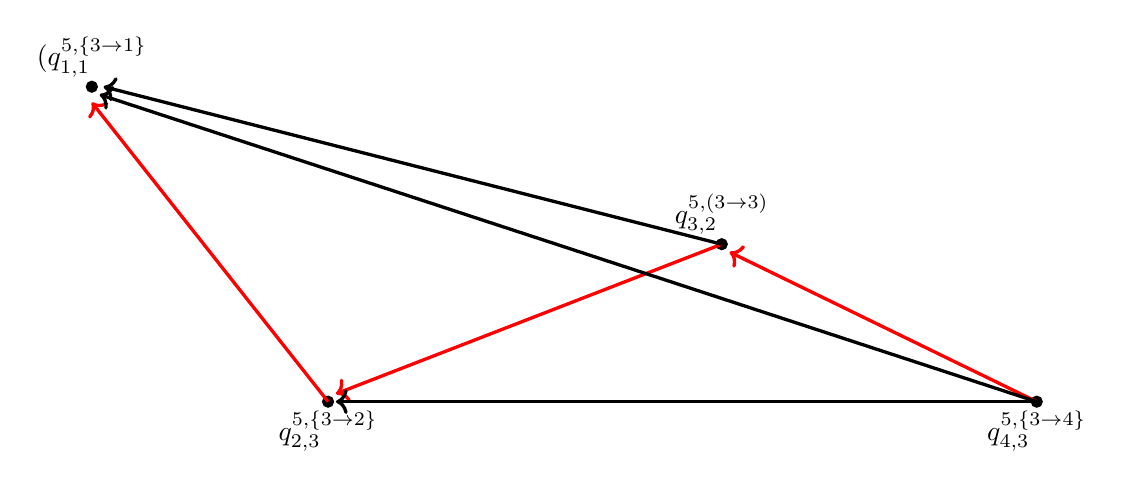
\begin{tikzpicture}
%%% The nodes represents the k query in the first round
\filldraw[black] (0, 4) circle (2pt) node [anchor=south]{$(q^{5, \{3 \to 1\}}_{1, 1}$};
% \filldraw[black] (8, 4) circle (2pt) node [anchor=south]{$\cdots$};
% \filldraw[black] (12, 4) circle (2pt) node [anchor=south]{$q^{1, (5, k)}_k$};
%%%%%% The nodes represents the n^k queries in the second round
% \filldraw[black] (0, 0) circle (2pt) node [anchor=north]{$q^{n!, (5, 1)}_1$};
\filldraw[black] (3, 0) circle (2pt) node [anchor=north]{$q^{5, \{3 \to 2\}}_{2, 3}$};
% \filldraw[black] (6, 0) circle (2pt) node [anchor=north]{$q^{3, 7}_{k+1}$};
% \filldraw[black] (8, 0) circle (2pt) node [anchor=north]{$\cdots$};
\filldraw[black] (12, 0) circle (2pt) node [anchor=north]{$q^{5, \{3 \to 4\}}_{4, 3}$};
%%% The nodes represents the k query in the first round
% \filldraw[black] (0, 2) circle (2pt) node [anchor=south]{$q^{\cdots, (5, 1)}_1$};
% \filldraw[black] (3, 2) circle (2pt) node [anchor=south]{$q^{\cdots, (5, 2)}_2$};
% \filldraw[black] (6, 2) circle (2pt) node [anchor=south]{$q^4_3$};
\filldraw[black] (8, 2) circle (2pt) node [anchor=south]{$q^{5, (3 \to 3)}_{3, 2}$};
% \filldraw[black] (12, 2) circle (2pt) node [anchor=south]{$q^{\cdots, (5, k)}_k$};
%%%%%% The edges represents their dependency relations GROUP 1
% \draw[very thick,->] (3, 2)  -- (0.1, 2) ;
% \draw[very thick,->] (3, 0)  -- (0.1, 1.9) ;
% \draw[very thick,->] (3, 4)  -- (0.1, 2.1) ;
% %
% \draw[very thick,->] (3, 2)  -- (0.1, 0.1) ;
% \draw[very thick,->] (3, 0)  -- (0.1, 0) ;
% \draw[very thick,->] (3, 4)  -- (0, 0.2) ;
% %
% \draw[very thick,->] (3, 2)  -- (0.1, 3.9) ;
\draw[very thick,->, red] (3, 0)  -- (0, 3.8) ;
% \draw[very thick,->] (3, 4)  -- (0, 4) ;
% \draw[very thick,->] (0, 0)  -- (6, 2) ;
%%%%%% The edges represents their dependency relations GROUP 2
% \draw[very thick,->] (0, 0)  -- (6, 2) ;
% \draw[very thick,->] (8, 2)  -- (3.1, 2) ;
% \draw[very thick,->] (8, 0)  -- (3.1, 1.9) ;
% \draw[very thick,->] (8, 4)  -- (3.1, 2.1) ;
%
\draw[very thick,->, red] (8, 2)  -- (3.1, 0.1) ;
\draw[very thick,->] (8, 2)  -- (0.15, 4) ;
% \draw[very thick,->] (8, 0)  -- (3.1, 0) ;
% \draw[very thick,->] (8, 4)  -- (3, 0.2) ;
% %
% \draw[very thick,->] (8, 2)  -- (3.1, 3.9) ;
% \draw[very thick,->] (8, 0)  -- (3, 3.8) ;
% \draw[very thick,->] (8, 4)  -- (3.1, 4) ;
%%%%%% The edges represents their dependency relations GROUP 4
% \draw[very thick,->] (0, 0)  -- (6, 2) ;
% \draw[very thick,->] (12, 2)  -- (8.1, 2) ;
\draw[very thick,->, red] (12, 0)  -- (8.1, 1.9) ;
\draw[very thick,->] (12, 0)  -- (3.1, 0) ;
\draw[very thick,->] (12, 0)  -- (0.1, 3.9) ;
% \draw[very thick,->] (12, 4)  -- (8.1, 2.1) ;
% %
% \draw[very thick,->] (12, 2)  -- (8.1, 0.1) ;
% \draw[very thick,->] (12, 0)  -- (8.1, 0) ;
% \draw[very thick,->] (12, 4)  -- (8, 0.2) ;
% %
% \draw[very thick,->] (12, 2)  -- (8.1, 3.9) ;
% \draw[very thick,->] (12, 0)  -- (8, 3.8) ;
% \draw[very thick,->] (12, 4)  -- (8.1, 4) ;
%
% \draw[very thick,->] (12, 2)  -- (8.1, 3.9) ;

%%%% The longest path representing the adaptivity
% \draw[ultra thick, red, ->, dashed] (3, 4.1)  -- (0.1, 4.1);
% \draw[ultra thick, red, ->, dashed] (8, 4.1)  -- (3.1, 4.1);
% \draw[ultra thick, red, ->, dashed] (12, 4.1)  -- (8.1, 4.1);
\end{tikzpicture}
\end{center}
%
%
$\forall k. \forall D$, we have $A(TR^L) = (k - 1)$ given all possible execution traces.
\begin{center}
%
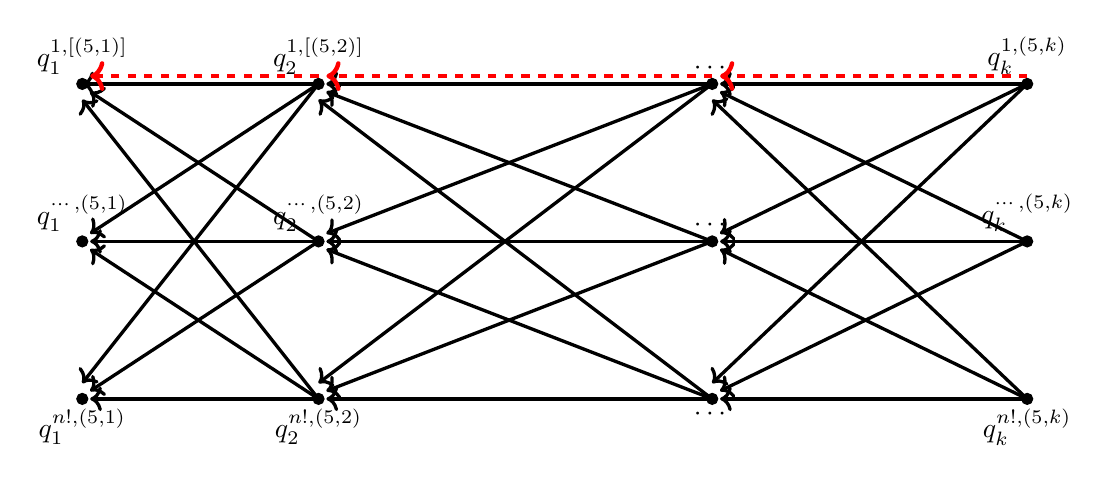
\begin{tikzpicture}
%%% The nodes represents the k query in the first round
\filldraw[black] (0, 4) circle (2pt) node [anchor=south]{$q^{1, [(5, 1)]}_1$};
\filldraw[black] (3, 4) circle (2pt) node [anchor=south]{$q^{1, [(5, 2)]}_2$};
% \filldraw[black] (6, 2) circle (2pt) node [anchor=south]{$q^4_3$};
\filldraw[black] (8, 4) circle (2pt) node [anchor=south]{$\cdots$};
\filldraw[black] (12, 4) circle (2pt) node [anchor=south]{$q^{1, (5, k)}_k$};
%%%%%% The nodes represents the n^k queries in the second round
\filldraw[black] (0, 0) circle (2pt) node [anchor=north]{$q^{n!, (5, 1)}_1$};
\filldraw[black] (3, 0) circle (2pt) node [anchor=north]{$q^{n!, (5, 2)}_2$};
% \filldraw[black] (6, 0) circle (2pt) node [anchor=north]{$q^{3, 7}_{k+1}$};
\filldraw[black] (8, 0) circle (2pt) node [anchor=north]{$\cdots$};
\filldraw[black] (12, 0) circle (2pt) node [anchor=north]{$q^{n!, (5, k)}_k$};
%%% The nodes represents the k query in the first round
\filldraw[black] (0, 2) circle (2pt) node [anchor=south]{$q^{\cdots, (5, 1)}_1$};
\filldraw[black] (3, 2) circle (2pt) node [anchor=south]{$q^{\cdots, (5, 2)}_2$};
% \filldraw[black] (6, 2) circle (2pt) node [anchor=south]{$q^4_3$};
\filldraw[black] (8, 2) circle (2pt) node [anchor=south]{$\cdots$};
\filldraw[black] (12, 2) circle (2pt) node [anchor=south]{$q^{\cdots, (5, k)}_k$};
%%%%%% The edges represents their dependency relations GROUP 1
\draw[very thick,->] (3, 2)  -- (0.1, 2) ;
\draw[very thick,->] (3, 0)  -- (0.1, 1.9) ;
\draw[very thick,->] (3, 4)  -- (0.1, 2.1) ;
%
\draw[very thick,->] (3, 2)  -- (0.1, 0.1) ;
\draw[very thick,->] (3, 0)  -- (0.1, 0) ;
\draw[very thick,->] (3, 4)  -- (0, 0.2) ;
%
\draw[very thick,->] (3, 2)  -- (0.1, 3.9) ;
\draw[very thick,->] (3, 0)  -- (0, 3.8) ;
\draw[very thick,->] (3, 4)  -- (0, 4) ;
% \draw[very thick,->] (0, 0)  -- (6, 2) ;
%%%%%% The edges represents their dependency relations GROUP 2
% \draw[very thick,->] (0, 0)  -- (6, 2) ;
\draw[very thick,->] (8, 2)  -- (3.1, 2) ;
\draw[very thick,->] (8, 0)  -- (3.1, 1.9) ;
\draw[very thick,->] (8, 4)  -- (3.1, 2.1) ;
%
\draw[very thick,->] (8, 2)  -- (3.1, 0.1) ;
\draw[very thick,->] (8, 0)  -- (3.1, 0) ;
\draw[very thick,->] (8, 4)  -- (3, 0.2) ;
%
\draw[very thick,->] (8, 2)  -- (3.1, 3.9) ;
\draw[very thick,->] (8, 0)  -- (3, 3.8) ;
\draw[very thick,->] (8, 4)  -- (3.1, 4) ;
%%%%%% The edges represents their dependency relations GROUP 4
% \draw[very thick,->] (0, 0)  -- (6, 2) ;
\draw[very thick,->] (12, 2)  -- (8.1, 2) ;
\draw[very thick,->] (12, 0)  -- (8.1, 1.9) ;
\draw[very thick,->] (12, 4)  -- (8.1, 2.1) ;
%
\draw[very thick,->] (12, 2)  -- (8.1, 0.1) ;
\draw[very thick,->] (12, 0)  -- (8.1, 0) ;
\draw[very thick,->] (12, 4)  -- (8, 0.2) ;
%
\draw[very thick,->] (12, 2)  -- (8.1, 3.9) ;
\draw[very thick,->] (12, 0)  -- (8, 3.8) ;
\draw[very thick,->] (12, 4)  -- (8.1, 4) ;
%
%%%% The longest path representing the adaptivity
\draw[ultra thick, red, ->, dashed] (3, 4.1)  -- (0.1, 4.1);
\draw[ultra thick, red, ->, dashed] (8, 4.1)  -- (3.1, 4.1);
\draw[ultra thick, red, ->, dashed] (12, 4.1)  -- (8.1, 4.1);
\end{tikzpicture}
\end{center}
\end{example}
%
%
\begin{thm}
[Observable Equivalent]
Given a program $P$ in high level language, the corresponding low level language $P^l$ rewrote from $P$ via the rewriting rules is observably equivalent to $P$.
\end{thm}
%
%
\subsection{Adaptivity of the High Level Language}
\begin{defn}
[Adaptivity]
Given a program $P$ in high level language, let $P^L$ be the set of all possible program in low level language observable equivalent to $P$, the adaptivity of $P$ is defined as:
\\
\[A(P) \triangleq \min\limits_{P^* \in P^L}A^*(P^*) \]
%
\end{defn}
%
%
\subsection{Soundness of \THESYSTEM ~ in High Level Language}
%
\begin{thm}
[Soundness]
Given a program $P$ in high level language, let $P^l$ be the corresponding program in low level rewrote from $P$ via the rewriting rules, 
then given $\Gamma$, $c_1$ and $c_2$ s.t. $\Gamma \subseteq FreeVar(P^l)$, 
$ \Gamma \vdash^{c_1, c_2}_{M,V} P^l $, then we have:
\\
\[Adaptivity(P) \leq Adapt(M,V) \]
\end{thm}
%
%
%
%
\clearpage
\section{Towards Probability}
%
\subsection{Syntax and Semantics}
%
\paragraph{Syntax.}
\[
\begin{array}{llll}
 \mbox{Arithmatic Operators} & *_a & ::= & + ~|~ - ~|~ \times 
%
~|~ \div \\  
  \mbox{Boolean Operators} & *_b & ::= & \lor \sep \land \\
   \mbox{Relational Operators} & *_r & ::= & < ~|~ \leq ~|~ = \\  
 \mbox{Label} & l & & \\ 
 \mbox{While Map} & w & \in & \mbox{Label} \times \mathbb{N} \triangleq w +l \sep w \setminus l \sep w \oplus_\rho w \\
\mbox{AExpr} & \aexpr & ::= & 
	%
	n ~|~ x ~|~ \aexpr *_a \aexpr ~|~ {[] ~|~ [\aexpr_0, \dots, \aexpr_i] \sep \aexpr \times \aexpr } \\
    %
\mbox{BExpr} & \bexpr & ::= & 
	%
	\etrue ~|~ \efalse  ~|~ \neg \bexpr
	 ~|~ \bexpr *_b \bexpr
	%
	~|~ \aexpr *_r \aexpr \\
\mbox{Deterministic Expr} & \expr_d & ::=	& \aexpr \sep \bexpr \\
\mbox{Randomized AExpr} & \aexpr_r & ::= & 
	%
	 x_r \sep n \sep  \aexpr_r *_a \aexpr_r \\
    %
\mbox{Randomized BExpr} & \bexpr_r & ::= & 
	%
\neg \bexpr_r
	 ~|~ \bexpr_r *_b \bexpr_r
	%
	~|~ \aexpr_r *_r \aexpr_r \\
\mbox{Randomized Expr} & \expr_r & ::=	& \expr_d \sep \aexpr_r \sep \bexpr_r \\
\mbox{Command} & \command & ::= &   [\assign x {\expr_d}]^{l} \sep [\assign {x_r} {\expr_r}]^{l} \sep  [\assign x q]^{l} \sep  [\assign {x_r} \uniform ]^{l} \sep   [\assign {x_r} \bernoulli]^{l} 
 %
\\
	%
& & & ~|~  \command ; \command  ~|~ \eif_D ([\bexpr]^{l}, \command_1, \command_2) \sep  \eif_R ([\bexpr_r]^{l}, \command_1, \command_2) 
 ~|~ [\eskip]^{l} \\
& & & { \sep [\eswitch( \expr, x, (v_i \to  q_i))]^{l}} \sep {\eloop ~ [\valr_N]^{l} ~ (f) ~ \edo ~ \command }
	\\
	%
% \mbox{Binary Operation} & \bop & ::= & + ~|~ - ~|~ \times 
% %
\mbox{Memory} & m & ::= & [] ~|~ m[x^{l} \to v] \\
%
\mbox{Trace} & t & ::= & [] ~|~ [(q, v)^{(l, w) }] ~|~ t ++ t 
~|~ t \oplus_{\rho} t
\end{array}
\]
%
\[
\begin{array}{ccl}
w \setminus l     & = &\left \{  
    \begin{array}{lr} w  & l \not\in Keys(w)   \\
      w_l & Otherwise \\
     \end{array} \right.\\
w + l & = &
 \left \{  
    \begin{array}{lr}
    w[l \to 0] & l \not \in Keys(w) \\   
    w_l [l \to w(l)+1] & Otherwise
          \end{array} \right.\\
\end{array}
\]
%
\paragraph{Semantics}
We have a countable set $\textsf{RV}$ of random variables($x_r \in \textsf{RV}$), a countable set $\textsf{Val}$ of values. For any subset  $\textsf{S} \subseteq \textsf{RV}$, we denote $\textsf{RanM[S]} \triangleq \textsf{S} \to \textsf{Val} $. We let $\textsf{DV}$ as a countable set of deterministic variables ($x$) and the deterministic memory $\textsf{DetM} \triangleq \textsf{DV} \to \textsf{Val}$. 
Distribution over A as $D(A)$. The \emph{distribution unit} unit : $A \to D(A)$. The \emph{distribution bind} bind : $ D(A) \to (A \to D(B)) \to D(B)$. $\lrr{C}{} : (\textsf{DetM} \times D(\textsf{RandM}) \times \textsf{Trace} \times \textsf{WhileMap} \times \textsf{DB} ) \to (\textsf{DetM} \times D(\textsf{RandM}) \times \textsf{Trace} \times \textsf{WhileMap} \times \textsf{DB} ) $

\[\config{(\sigma, \mu_1 , t_1, w_1, D)} \oplus_{\rho} \config{(\sigma, \mu_2 , t_2, w_2, D)} 
\triangleq \config{\sigma, \mu_1\oplus_{\rho} \mu_2 , t_1\oplus_{\rho} t_2, w_1 \oplus_{\rho} w_2, D}\]
%
\[(t_1 \oplus_{\rho} t_2)  ++ t_3 \triangleq 
(t_1 ++ t_3) \oplus_{\rho} (t_2 ++ t_3) \]
%
\[t_3 ++ (t_1 \oplus_{\rho} t_2) \triangleq 
(t_3 ++ t_1) \oplus_{\rho} (t_3 ++ t_2) \]
%
\[ (w_1 \oplus_{\rho} w_2) + l \triangleq 
(w_1 + l) \oplus_{\rho} (w_2 + l) \]
%
\[ (w_1 \oplus_{\rho} w_2) \setminus l \triangleq 
(w_1 \setminus l) \oplus_{\rho} (w_2 \setminus l) \]
\begin{figure}[H]%
    \centering
    \[
    \begin{array}{rll}
        \lrr{ [\eskip]^{l} }{} (\sigma, \mu , t, w, D) & \triangleq & (\sigma, \mu , t, w , D)  \\
        \lrr{ [\assign x {\expr_d}]^{l} }{} (\sigma, \mu , t, w, D)  & \triangleq & (\sigma[x \to \lrr{\expr_d}{}(\sigma)], \mu , t, w, D) \\
        \lrr{ [\assign {x_r} {\expr_r}]^{l}}{} (\sigma, \mu , t, w, D)  & \triangleq & (\sigma, bind(\mu , m \to unit(m[x_r \to \lrr{\expr_r}{}(\sigma, m)]) ) , t, w , D ) \\
        \lrr{ [\assign x q]^{l} }{} (\sigma, \mu , t, w, D)  & \triangleq & (\sigma[x \to v ], \mu , t ++ [(q, v)]^{(l, w)}, w , D) \qquad : v = q(D)\\
        \lrr{ [\assign {x_r} \uniform ]^{l} }{} (\sigma, \mu , t, w, D)  & \triangleq & (\sigma,  bind(\mu , m \to bind(\uniform , u \to m[x_r \to u] ) )  , t, w, D) \\
        \lrr{ [\assign {x_r} \bernoulli ]^{l} }{} (\sigma, \mu , t, w , D)  & \triangleq & (\sigma , bind(\mu , m \to bind(\bernoulli , u \to m[x_r \to u] ) ) , t, w,D) \\
            \lrr{ \command ; \command' }{} (\sigma, \mu , t, w , D)  & \triangleq & \lrr{\command'}{} ( \lrr{\command}{} \sigma , \mu, t, w) \\
         \lrr{ \eif_D ([\bexpr]^{l}, \command_1, \command_2)  }{} (\sigma, \mu , t, w , D)  & \triangleq & \left \{  \begin{array}{l} 
         \lrr{\command_1}{} (\sigma , \mu, t, w, D) \qquad : \lrr{\bexpr}{}(\sigma) = \etrue \\ 
         \lrr{\command_1}{} (\sigma , \mu, t, w,D) \qquad : \lrr{\bexpr}{}(\sigma) = \efalse \end{array} \right . \\    
           \lrr{ \eif_R ([\bexpr_r]^{l}, \command_1, \command_2)  }{} (\sigma, \mu , t, w , D)  & \triangleq & \left \{
           \begin{array}{l}
           \lrr{\command_1}{} (\sigma , \mu | \lrr{\bexpr_r}{} \sigma = \etrue  , t, w, D) \oplus_\rho  \lrr{\command_2}{} (\rho , \mu | \lrr{\bexpr_r}{} \sigma = \efalse  , t, w,D)  \\ 
           \lrr{\command_1}{} (\sigma , \mu | \lrr{\bexpr_r}{} \sigma = \etrue  , t, w, D) \qquad \rho = 1 \\
           \lrr{\command_2}{} (\sigma , \mu | \lrr{\bexpr_r}{} \sigma = \efalse  , t, w,D) \qquad \rho = 0 \\
            \end{array} \right . \\
             & & \textsf{where} \quad \rho = \mu (\lrr{\bexpr_r}{} \sigma = \etrue ) \\
        %   \lrr{ \ewhile([\bexpr]^{l}, \command) }{} (\sigma, \mu , t, w , D)  & \triangleq & \lrr{\eunfold{[\bexpr]^{l}}{ \ewhile([\bexpr]^{l}, \command) }   }{} (\sigma, \mu , t, w , D) \\
        %   \lrr{ \eunfold{[\bexpr]^{l}}{\command}  }{} (\sigma, \mu , t, w , D)  & \triangleq & \left \{  \begin{array}{l} \lrr{\command}{} (\sigma , \mu, t, w + l, D) \qquad : \lrr{\bexpr}{}(\sigma) = \etrue \\ \lrr{\eskip}{} (\sigma , \mu, t, w-l, D) \qquad : \lrr{\bexpr}{}(\sigma) = \efalse \end{array} \right . \\  
           \lrr{ {[\eswitch( \expr, x, (v_i \to  q_i))]^{l}} }{} (\sigma, \mu , t, w , D)  & \triangleq & 
          \lrr{ [\assign x q_1]^{l} }{} ( \sigma, \mu , t, w, D ) 
          \qquad : v_1 = \lrr{\expr}{}{(\sigma)} \\ 
           \lrr{ {\eloop ~ [\expr_N]^{l} ~ (f) ~ \edo ~ \command } }{} (\sigma, \mu , t, w , D)  & \triangleq & \left \{  \begin{array}{l} \lrr{f;\command; \eloop ~ [\expr_N-1]^{l} ~ (f) ~ \edo ~ \command }{} (\sigma , \mu, t, w + l, D) \qquad : \lrr{\expr_N}{}(\sigma) >0 \\ \lrr{\eskip}{} (\sigma , \mu, t, w-l, D) \qquad : \lrr{\expr_N}{}(\sigma) = 0 \end{array} \right . \\  
    \end{array}
    \]
    \caption{Semantics of programs}
    \label{fig:semantics_prob}
\end{figure}
%
%
% \[
% \begin{array}{l}
%      \left[j \leftarrow 0 \right]^1 ; \\
%     \left[I \leftarrow [] \right]^2; \\
%     \ewhile \Big( 
%     \left[j \leq k \right]^3 , \\
%     \left[p \leftarrow 0 \right]^4 ; \\
%     \left[
%     \eswitch \Big( I, x
%     \left(\begin{array}{l}
%         [ ] \to q_{j,1},\\
%         \cdots\\
%     \clabel{1, 2, 3, \cdots, n} \to q_{j,n!}
%     \end{array}\right)
%     \Big)
%     \right]^5\\
%     \clabel{I \leftarrow \eupdt(I, (x, p))}^6;\\
%     \clabel{j \leftarrow j + 1 }^7
%     \Big) ;
% \end{array}
% %
% ~~~~ \Rightarrow ~~~
% %
% SSA \triangleq
% \begin{array}{l}
%      \left[j \leftarrow 0 \right]^1 ; \\
%     \left[I_1 \leftarrow [] \right]^2; \\
%     \ewhile \Big( 
%     \left[j \leq k \right]^3 , \phi: {I_2} = f({I_1}, {I_3}) \\
%     \left[p \leftarrow 0 \right]^4 ; \\
%     \left[
%     \eswitch \Big( {I_2}, x
%     \left(\begin{array}{l}
%         [ ] \to q_{j,1},\\
%         \cdots\\
%     \clabel{1, 2, 3, \cdots, n} \to q_{j,n!}
%     \end{array}\right)
%     \Big)
%     \right]^5\\
%     \clabel{{I_3} \leftarrow \eupdt({I_2}, (x, p))}^6;\\
%     \clabel{j \leftarrow j + 1 }^7
%     \Big) ;
% \end{array}
% \]
% %
%
\subsection{Extending Adaptivity onto Probabilistic Program}
%
\begin{defn}
Dependency Forest.
\\
Given a program $P$, a database $D$, 
dependency forest $F(P, D) \triangleq \{ G_1, G_2, \cdots, G_m \}$,
$G_k = (V_k, E_k)$ is defined as: 
\\
$V_k =\{q^{l,w} |\forall m, w. \config{\emptyset, P, D,[], \emptyset } \rightarrow \config{m, \eskip, D, T, \emptyset} \land q^{l,w} \in \pi_k (T)  \}$;
\\
$E_k = \left\{(q_i^{l,w},q_j^{l',w'}) 
~ \left \vert ~ \neg \mathsf{IND}(q_i^{l,w},q_j^{l',w'}, P)
\land \mathsf{To}(q_j^{l',w'}, q_i^{l,w}) \right.\right\}$,
\\
where $\pi_k (T) = t_k$ s.t. $T = t_1 \oplus_{\rho_1} t_2 \oplus_{\rho_2}
\cdots \oplus_{m - 1} t_m $ and there is no $\oplus$ in $t_i$.
\end{defn}

\begin{defn}
Dependency Graph.
\\
Given a program $P$, a database $D$, 
dependency graph $G(P, D) \triangleq (V, E)$ is defined as: 
\\
$V =\bigcup \{V_k | G_k \in F(P, D)  \}$;
\\
$E_k = \left\{(q_i,q_j) 
~ \left \vert ~ (q_i,q_j) \in E_k , G_k \in F(P, D) \right.\right\}$,
\end{defn}
%
%
\begin{defn}
Adaptivity.
\\
Given a program $P$ and for all the database $D$ in a set of $DBS$ of databases, the total dependency graph G is the combination of all the dependent graphs over every single database $G(P, D) = (V, E)$, the adaptivity of the program is defined as $A(P)$, s.t.:
for every pair $(i,j)$ let $p_{(i,j)}$ be the longest path starting from $q_i^{l, w}$ to $q_j^{l',w'}$,
%
$$A(P) = \max\limits_{q_i^{l,w},q_j^{l',w'} \in V }\{l_i ~|~ l_i = |p_(i,j)| \}$$
\end{defn}
%
%
\section{Analysis of Generalization Error}

\begin{example}[Two Round Algorithm]
\[
TR^H(k) \triangleq
{
\begin{array}{l}
    % \left[j \leftarrow 0 \right]^1 ; \\
    \clabel{a_1 \leftarrow [] }^1; \\
    \eloop ~ [k]^{2} ~ (a_2 \leftarrow f(1, a_1, a_3)) \\
    ~ \edo ~ \\
    \Big(
     \clabel{x_1 \leftarrow q() }^3 ; \\
    \clabel{a_3 \leftarrow x_1 :: a_2 }^4     \Big);\\
    \clabel{l \leftarrow q_{k + 1}(a_3)}^{5}\\
\end{array}
}
\]
\end{example}
%
\begin{example}[Multi-Round Algorithm]
\[
MR^H \triangleq
\begin{array}{l}
    %  \left[j \leftarrow 0 \right]^1 ; \\
    \left[I_2 \leftarrow [] \right]^1; \\
    \eloop ~ [k]^{2} ~ (I_2 \leftarrow f(2, I_1, I_3)) \\ 
    \ ~ \edo ~ \\ \Big(
    \left[p_1 \leftarrow c \right]^3 ; \\
    \left[a_1 \leftarrow \delta(q(p, I_2)) \right]^4; \\
    \left[I_3 \leftarrow \eupdt( {I_2}, (a_1, p))  \right]^5
    \Big) 
\end{array}
\]
\end{example}
%
%
By applying different mechanisms $\delta()$ over the queries $q(\cdot)$, we have different error bounds.
\\
\textbf{Gaussian Mechanism:} $N(0, \sigma)$ \cite{dwork2015preserving}:
\\
Adaptivity $r = 2$: 
$ \sigma = O \left(\frac{\sqrt{r \log(k)}}{\sqrt{n}} \right)$ (also known as expected error);
\\
Adaptivity unknown:
$ \sigma = O\left(\frac{\sqrt[4]{k}}{\sqrt{n}} \right)$;
\\
{Mean Squared Error Bound:} 
$ \frac{1}{2n} \min\limits_{\lambda \in [0, 1]}
\left( \frac{2\rho k n - \ln(1 - \lambda)}{\lambda} 
\right)
+ 2 \mathbb{E}_{Z_i \sim N(0, \frac{1}{2n^2 \rho})}
\left[ \max\limits_{i \in [k]} (Z_i^2) \right]$
%
\\
{Confidence Bounds:} minimize $\tau$ where
$\tau \geq \sqrt{\frac{2}{n \beta}
\min\limits_{\lambda \in [0, 1]}
\left( \frac{2\rho k n - \ln(1 - \lambda)}{\lambda} 
\right)
}$
and 
$\tau \geq \frac{2}{n} \sqrt{\frac{\ln(4n /\beta}{\rho'}}$ with confidence level $1 - \beta$ .
\\
\textbf{$(\epsilon, \delta)-DP$ mechanism}:
\\
Confidence Bounds:
$\tau \geq \sqrt{\frac{48}{n} \ln(4/\beta) }$ with $\epsilon \leq \frac{\tau}{4}$ and $\delta = 
\exp \left(\frac{-4 \ln (8/\beta)}{\tau} \right)$
\\
\textbf{Sample Splitting}: 
\\
Expected Error: $O \left(\frac{\sqrt{k \log(k)}}{\sqrt{n}} \right)$
\\
\textbf{Thresholdout}: $B, \sigma, T, h$ 
\\
Confidence bounds:  
$\tau = \max\limits\left\{ 
\sqrt{\frac{2\zeta }{h \beta}},
2\sigma \ln(\frac{\beta}{2}),
\sqrt{\frac{1}{\beta}} \cdot \left(\sqrt{T^2 + 56\sigma^2} + \sqrt{\frac{\zeta}{4h} } \right)
\right\}
$,
for $\zeta = \min\limits_{\lambda \in [0, 1)}
\left( \frac{2B \ (\sigma^2 h) - \ln(1 - \lambda)}{\lambda} \right)$
%


\newpage
\section{Related Work}


\subsection{History of Program Dependency Graph and Relevant Graph}
First data flow computation: 

\cite{dennis1974preliminary} is the first version of the data flow procedure language, as well as \cite{dennis1980data}. They all give the computation for program's data flow.

\cite{davis1982data} then gave the analysis of the control flow and graph by converting the control flow into data flow.
\cite{allen1987automatic} , \cite{allen1983dependence} and \cite{scarborough1986vectorizing} proposed the approach of converting control dependence to data dependence named vectorization.
And then, \cite{treleaven1982combining} firstly combined the data flow with the control flow and give a comprehensive analysis.

Combing the data and control flow analysis, \cite{towle1976control} gave the data dependence graph in his thesis by analyzing the control and data dependence for program transformation.

Then based on both the data and control dependence graphs, \cite{kuck1972number}, \cite{kuck1981dependence} and \cite{baxter1989program} firstly gave the program dependence graph, which analyzing the programs aims to the program parallelism. 
This is also extensively studied in \cite{ferrante1983program}, \cite{ferrante1987program}  and \cite{ferrante1985linearizing}. 
Following this line of work, the program dependence graph was then applied into the program optimization and software development environment in \cite{ottenstein1984program} and \cite{ferrante1987program}.

 


\subsection{Dynamic Program Graph Analysis}

\cite{sinha2001interprocedural}: 
Support Interprocedural Control dependence analyzing, semantically.
\\
They identified the dependence information between the interactions of among procedures, specifically the control dependence between procedures.
Their analysis support the relationship of control and data dependence to semantics dependence.

\cite{austin1992dynamic}: Dynamic Program Dependency Graph.
\\
They gave the dynamic analysis for the program's dependency, by producing 3 different kinds of graph, 
including the data flow graph, storage dependence and control dependence graph from program's execution traces. 
\\
Then, they constructing dynamic execution graphs by adopting the 3 graph, aims to expose the parallization of the programs

\cite{hammer2006dynamic}: dynamic path conditions in dependence graphs.
They adopting the dynamic information from program trace to the path condition in dependency graph. Then based on these information, 
they present new approach combining dynamic slicing, which could reveal both dependences holding during program execution as well as why these dependences are holding. 
Aims to have a finer and preciser analysis of the program.

\subsection{Utilization of the Dynamic Program Dependency}

\cite{nagar2018automated}: Utilize dependency graph for finding serializability violation. 
\\
Combine with the dependency graph of serialization and abstract execution, to statically finding bounded serializability violation. 
Then reduce the problem of serializability to satisfiability of a formula in FOL.
Also reason about unbounded executions.

\subsection{Static Program Dependency}

\cite{mastroeni2008data}: They propose ways of constructing different kinds of program slices, by choose different program dependency. For example, in either syntactic or semantics sense.
This abstract dependency is based on properties rather than exact data.
Aims to give finer and smaller program slice. 

\subsection{Utilization Static Program Flow Graph}

\cite{arlt2012lightweight}: Lightweight Static Analysis for GUI Testing. They give the relevant event graph based on black and white Box.
To construct finer Event Sequence Graph, 
they propose new approach to select relevant event sequences among the event sequences generated by black box.
This new approach based on static analysis on bytecode of the applications, 
giving a precisely defined dependency between a fixed number of events in event sequence.
Then, they inferred a finer Event Dependency graph, aims to give a better lightweight static analysis on applications.




\newpage
\bibliographystyle{alpha}
\bibliography{adaptivity.bib}

\end{document}



